% -----------------------------------------  
% Autogenerated LaTeX file from XML DocBook  
% -----------------------------------------  
%%<params>
%%</params>
\documentclass{report}
\usepackage{ifxetex}
\ifxetex
\usepackage{fontspec}
\usepackage{xltxtra}
\setmainfont{DejaVu Serif}
\setsansfont{DejaVu Sans}
\else
\usepackage[T1]{fontenc}
\usepackage[latin1]{inputenc}
\fi
\usepackage{fancybox}
\usepackage{makeidx}
\usepackage[hyperlink]{docbook}
\renewcommand{\DBKreleaseinfo}{}
\setcounter{tocdepth}{5}
\setcounter{secnumdepth}{5}
\title{D2.1a -{} VISHNU User Management System Package Design}
\author{Benjamin Isnard, Daouda Traor�, Eug�ne Pamba Capo-{}Chichi, Kevin Coulomb, and Ibrahima Ciss�}
\hypersetup{%
pdfcreator={DBLaTeX-0.2.9-3},%
pdftitle={D2.1a -{} VISHNU User Management System Package Design},%
pdfauthor={Benjamin Isnard, Daouda Traor�, Eug�ne Pamba Capo-{}Chichi, Kevin Coulomb, and Ibrahima Ciss�}%
}
% ------------------
% Collaborators
% ------------------
\renewcommand{\DBKindexation}{
\begin{DBKindtable}
\DBKinditem{\writtenby}{Benjamin Isnard, Daouda Traor�, Eug�ne Pamba Capo-{}Chichi, Kevin Coulomb, and Ibrahima Ciss�}
\end{DBKindtable}
}
\makeindex
\makeglossary

%% ----------------------
%% Revision History Table
%% ----------------------
\renewcommand{\DBKrevhistory}{
\begin{DBKrevtable}
~\par
1~\par

& ~\par
25/01/2011
& ~\par
   
Deliverable version

& ~\par
SysFera
\tabularnewline
\hline

\end{DBKrevtable}}

    \begin{document}
\frontmatter
\maketitle
\tableofcontents
\listoffigures
\mainmatter

% ------- 
% Chapter 
% ------- 

\chapter{Document presentation}

\section{Document objectives}

This document presents the detailed internal design of the Users Management System (UMS) package. The purpose of this
        package is to handle all aspects of user management and session management within the VISHNU system. The functional
        and non-{}functional requirements for this package are those described in the referenced specification documents. The current
        document is part of the design phase of the software and therefore its main goal is to define the main components of the
        system architecture and their relationships.
 

\section{Document structure}

\begin{itemize}

\item{}Chapter 1 contains a brief overview of the document content.


\item{}Chapter 2 contains a high-{}level overview of the system architecture.


\item{}Chapter 3 describes the internal API used for remote procedure calls through SysFera-{}DS.


\item{}Chapter 4 describes the internal class and data structures

\end{itemize}


\section{References}

\begin{itemize}

\item{}[D1.1a]: VISHNU General specifications


\item{}[D1.1b]: VISHNU Sp�cifications techniques des besoins


\item{}[D1.1c]: VISHNU API Detailed specifications

\end{itemize}


\section{Acronyms}

  \begin{itemize}

\item{}\textbf{API}: Application programming interface


\item{}\textbf{CLI}: Command line interface


\item{}\textbf{DB}: DataBase


\item{}\textbf{n/a}: Not Appliable (used for serializable capability in function descriptions)


\item{}\textbf{SeD}: A Server Daemon is a SysFera-{}DS agent that provides services through the SysFera-{}DS API.


\item{}\textbf{UMS}: Users management system


\item{}\textbf{WS}: Web services

\end{itemize}
  

\section{Glossary}

  \begin{itemize}

\item{}\textbf{Components}: the software components represents a library or an executable program that provides a given interface to other components or to end-{}users.


\item{}\textbf{Serialized type}: this is a class of data (C++ Class) which instances can be serialized in a XML string before being sent over an API (to or from the API). The data is deserialized on the other side of the channel in order to re-{}build the same instance of the class.


\item{}\textbf{SysFera-{}DS}: open-{}source middleware developped by SysFera.

\end{itemize}
  

% ------- 
% Chapter 
% ------- 

\chapter{System Architecture}

\section{Overview of the UMS software infrastructure}

We present in this section a detailed description of the UMS package architecture in terms of software components.
	In addition we show the dependencies between components to highlight their reuse. These components follow a client/server model.
        We present the different software layers from services (provided directly to the user) to the database (used by the server). 
	The UMS client server package has been split into eight different interrelated components. The diagrams shown in section 2.3 describe
        the relationships between these components. The definitions of the components are the following:
 

  \begin{itemize}

\item{}\textbf{External API} 	     contains precisely the services provided to the user as defined in the detailed specifications.
	     We're on the client side.
 


\item{}\textbf{Internal API} 	     is the middle layer of the server side. The services announced previously are performed here by combining a set of classes defined 
	    in the two following components.
 


\item{}\textbf{UMS Client} 	    contains intermediate (proxy) classes providing remote access to the business objects of \textbf{UMS Server}.
 


\item{}\textbf{UMS Server} 	     contains all classes implementing business objects by encapsulating the processing provided through the internal API.
 


\item{}\textbf{Sysfera-{}DS Client API} is the C++ client API provided by the SysFera-{}DS toolbox.


\item{}\textbf{Sysfera-{}DS Server API} is the C++ server API provided by the SysFera-{}DS toolbox.


\item{}\textbf{UMS Monitor Daemon} which the only role is to keep an eye on the session inactivity by checking the TIME\_OUT parameter in the \textbf{Vishnu Database.}  


\item{}\textbf{Vishnu Database} stores all data manipulated by the UMS Server.
 

\end{itemize}
  

\section{ Deployment aspects of UMS}

         We explains here how the UMS package will be deployed in a physical hardware as illustrated in figure 2.1  where each cube represents an environement in which a component or a set of components execute. The UMS consists of: 
 \begin{itemize}

\item{}\textbf{ Main UMS Server }is the provider of all UMS services. It consists of the UMS Monitor component and what we called the UMS SeD (UMS Server daemon) which gathers all UMS services published.
 


\item{}\textbf{Secondary UMS Server } is optional and contains only the UMS SeD allowing to make a UMS service request.  
 


\item{}\textbf{Client host } is UMS service requester. It contains all components allowing to make a UMS service request.	  
 


\item{}\textbf{SysFera-{}DS Bus } is the specific software layer that ensures the communication between client hosts and server hosts. 
 


\item{}\textbf{Vishnu database}: this component represents a unique instance of an Oracle or PostgreSQL database.
 

\end{itemize}
  

 It is important to note that we can have several Secondary UMS servers (where an UMS Sed is running in each) but only one instance of UMS Monitor daemon running in the Main UMS Server as we can see in figure 2.1.
 

\section{Architecture diagrams}

\subsection{UMS Deployment Diagram}

This diagram shows the classes of entities that must be deployed for the Vishnu UMS application to work. One Main UMS Server contains both a UMS SeD component and a UMS Monitor Daemon component. The Secondary UMS Server entity is optional and can be duplicated to improve performance and robustness. All UMS Server entities connect to the same Vishnu database. It is important to note that the different classes are here shown on different nodes but they can also be deployed on the same node.
\begin{figure}[H]

\begin{center}
\imgexists{images/png/UMS_Deployment_Diagram.png}{{\centering \imgevalsize{images/png/UMS_Deployment_Diagram.png}{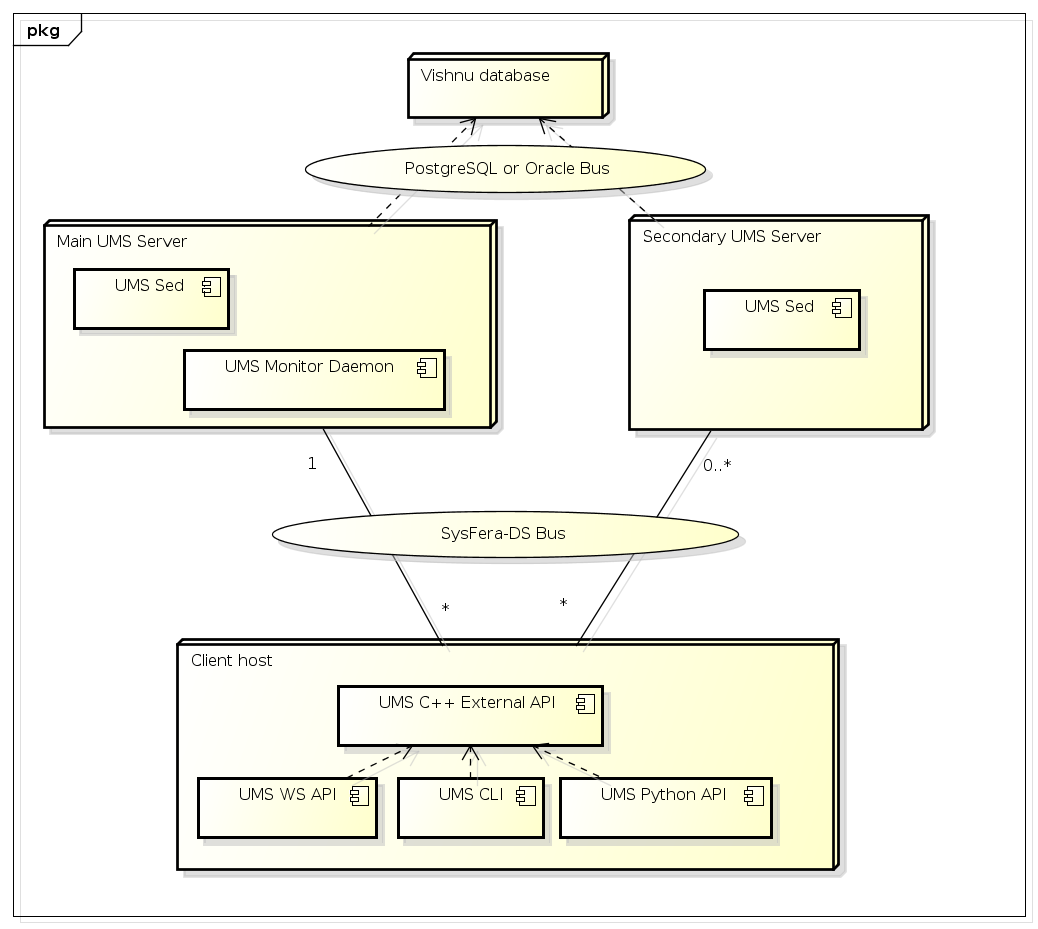
\includegraphics[scale=0.4]{images/png/UMS_Deployment_Diagram.png}}}}{}
\end{center}
\caption{UMS Deployment Diagram}
\end{figure}

\subsection{UMS client-{}side components}

This diagram shows the components that compose the client side of the Vishnu UMS system and their interfaces. Two services among all the services of the UMS external API (see ref. D1.1c) are shown here for example. These services are consumed by several user interfaces: command-{}line, web services and Python. All the interfaces of the UMS Client component are shown.
\begin{figure}[H]

\begin{center}
\imgexists{images/png/UMS_client-side_components.png}{{\centering \imgevalsize{images/png/UMS_client-side_components.png}{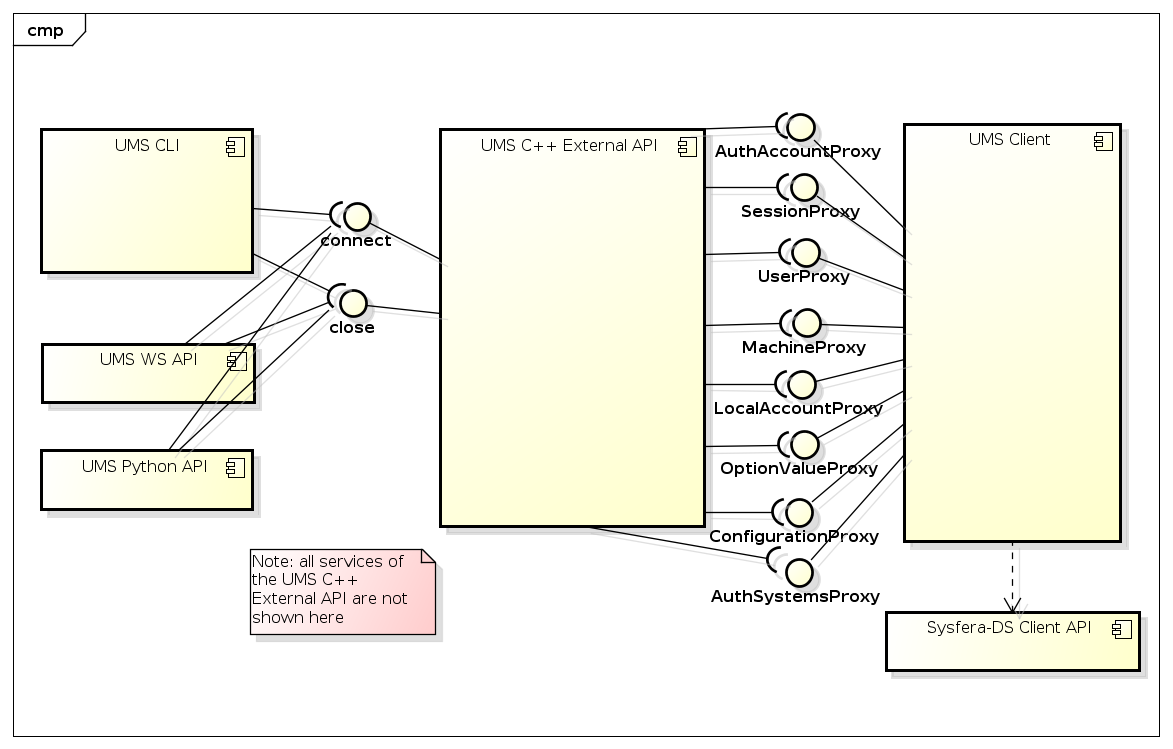
\includegraphics[scale=0.4]{images/png/UMS_client-side_components.png}}}}{}
\end{center}
\caption{UMS client-{}side components}
\end{figure}

\subsection{UMS server-{}side components}

This diagram shows the components that compose the server side of the Vishnu UMS system and their interfaces. Two services among all the services of the UMS internal API are shown here for example. These services are consumed by the UMS Client component through the SysFera-{}DS API. All the interfaces of the UMS Server component are shown.
\begin{figure}[H]

\begin{center}
\imgexists{images/png/UMS_server-side_components.png}{{\centering \imgevalsize{images/png/UMS_server-side_components.png}{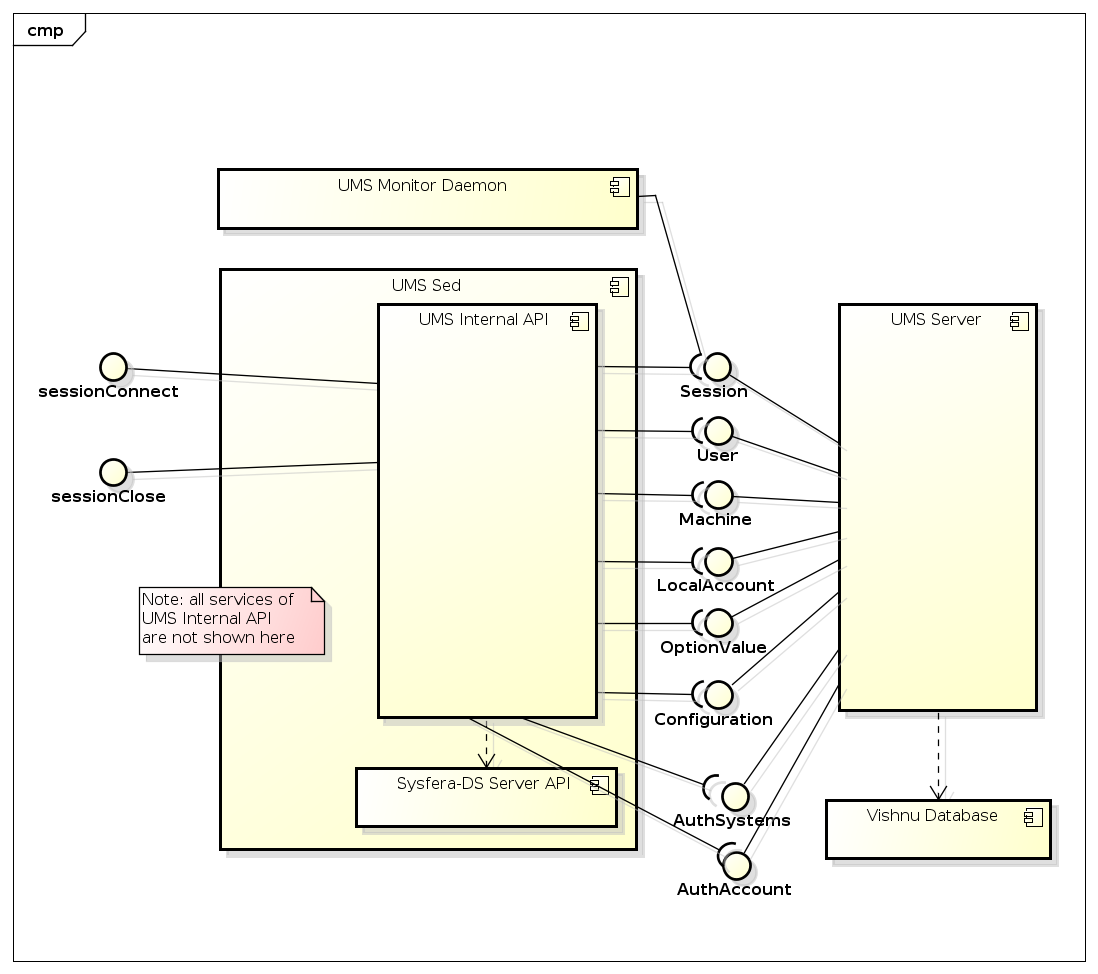
\includegraphics[scale=0.4]{images/png/UMS_server-side_components.png}}}}{}
\end{center}
\caption{UMS server-{}side components}
\end{figure}

\subsection{SysFera-{}DS Bus Details}

This diagram shows the communication paths between the Client host and the UMS Main and Secondary server using the SysFera-{}DS Bus. The SysFera-{}DS MasterAgent is a SysFera-{}DS agent that can be executed on a dedicated host or on the same host as the UMS Server. All the communications between the entities here are done using the CORBA IIOP (Internet Inter-{}ORB) protocol and the communications can be tunneled through SSH tunnels if necessary. The MasterAgent entity is involved in the choice of one UMS Server in the case of  several available UMS servers. The choice will be transparent to the user as all UMS Servers connect to the same database.  The diagram shows here all the communication paths in the case where the Main UMS Server is chosen by the MasterAgent.
\begin{figure}[H]

\begin{center}
\imgexists{images/png/SysFera-DS_Bus_Details.png}{{\centering \imgevalsize{images/png/SysFera-DS_Bus_Details.png}{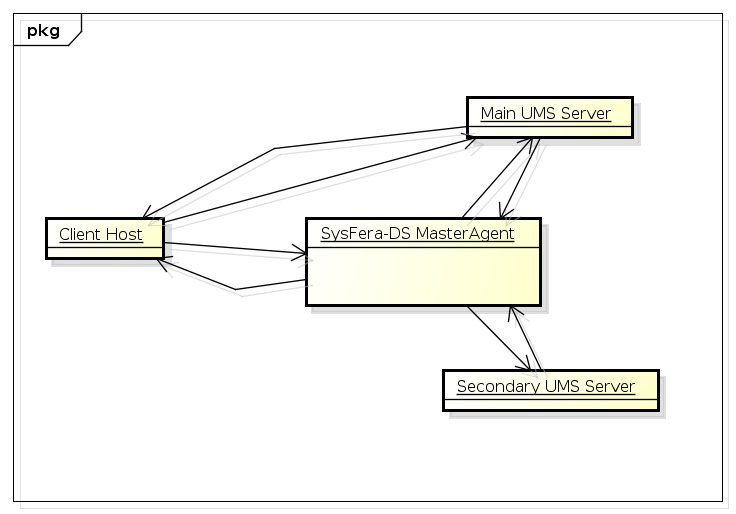
\includegraphics[scale=0.4]{images/png/SysFera-DS_Bus_Details.png}}}}{}
\end{center}
\caption{SysFera-{}DS Bus Details}
\end{figure}

% ------- 
% Chapter 
% ------- 

\chapter{Internal API specification}

\section{Generic definition formats presentation}

This section presents the formats used in this chapter to describe the services provided
            by the internal API.

\subsection{Service definition format}

\textbf{Access }

Here is detailed the access level of the service 'myService' (i.e. the privilege required to use it)

\textbf{Parameters}

The following table contains all the input and output parameters of the service, along with their type and description.

{\centering \savetablecounter \begingroup%
\setlength{\newtblsparewidth}{\linewidth-2\tabcolsep-2cm-2\tabcolsep-2cm-2\tabcolsep-3cm-2\tabcolsep-8cm-2\tabcolsep-1cm-2\tabcolsep}%
\begin{longtable}{lllll}\hline
\multicolumn{1}{|m{2cm}|}{\raggedright\bfseries%
%
Parameter%
}&\multicolumn{1}{m{2cm}|}{\raggedright\bfseries%
%
Type%
}&\multicolumn{1}{m{3cm}|}{\raggedright\bfseries%
%
Serialized type%
}&\multicolumn{1}{m{8cm}|}{\raggedright\bfseries%
%
Description%
}&\multicolumn{1}{m{1cm}|}{\raggedright\bfseries%
%
Mode%
}\tabularnewline
\cline{1-1}\cline{2-2}\cline{3-3}\cline{4-4}\cline{5-5}\endhead
\multicolumn{1}{|m{2cm}|}{\raggedright%
sessionKey
%
}&\multicolumn{1}{m{2cm}|}{\raggedright%
string
%
}&\multicolumn{1}{m{3cm}|}{\raggedright%
n/a
%
}&\multicolumn{1}{m{8cm}|}{\raggedright%
This is an example of a required string input parameter
%
}&\multicolumn{1}{m{1cm}|}{\raggedright%
IN
%
}\tabularnewline
\cline{1-1}\cline{2-2}\cline{3-3}\cline{4-4}\cline{5-5}\multicolumn{1}{|m{2cm}|}{\raggedright%
listOfJobs
%
}&\multicolumn{1}{m{2cm}|}{\raggedright%
string
%
}&\multicolumn{1}{m{3cm}|}{\raggedright%
ListJobs
%
}&\multicolumn{1}{m{8cm}|}{\raggedright%
This is an example of an object output parameter that is serialized as a string
%
}&\multicolumn{1}{m{1cm}|}{\raggedright%
OUT
%
}\tabularnewline
\hline
\end{longtable}\endgroup%
\restoretablecounter%
}

\textbf{Description }

Here is detailed the purpose of the service 'myService'

\textbf{Return Value }

Here are detailed the different return codes provided by the service.

{\centering \savetablecounter \begingroup%
\setlength{\newtblsparewidth}{\linewidth-2\tabcolsep-8.5cm-2\tabcolsep-9cm-2\tabcolsep}%

\begin{longtable}{ll}\hline
\multicolumn{1}{|m{8.5cm}|}{\raggedright\bfseries%
%
Name%
}&\multicolumn{1}{m{9cm}|}{\raggedright\bfseries%
%
Description%
}\tabularnewline
\cline{1-1}\cline{2-2}\endhead
\multicolumn{1}{|m{8.5cm}|}{\raggedright%
VISHNU\_OK
%
}&\multicolumn{1}{m{9cm}|}{\raggedright%
The service has been performed successfully.
%
}\tabularnewline
\cline{1-1}\cline{2-2}\multicolumn{1}{|m{8.5cm}|}{\raggedright%
TMS\_UNKNOWN\_MACHINE
%
}&\multicolumn{1}{m{9cm}|}{\raggedright%
This is the human-{}readable generic message that will be available to the user of the API.
%
}\tabularnewline
\hline
\end{longtable}\endgroup%
\restoretablecounter%
}

\textbf{Used by this(these) API function(s): }

This shows the list of functions from the external Vishnu API (see [D1\_1c]) that use this service.

\section{Definition of the services of the package}

\subsection{Service commandList}

\textbf{Access}

This service can be used by any VISHNU user

\textbf{Parameters}

{\centering \savetablecounter \begingroup%
\setlength{\newtblsparewidth}{\linewidth-2\tabcolsep-2cm-2\tabcolsep-2cm-2\tabcolsep-3cm-2\tabcolsep-8cm-2\tabcolsep-1cm-2\tabcolsep}%

\begin{longtable}{lllll}\hline
\multicolumn{1}{|m{2cm}|}{\raggedright\bfseries%
%
Parameter%
}&\multicolumn{1}{m{2cm}|}{\raggedright\bfseries%
%
Type%
}&\multicolumn{1}{m{3cm}|}{\raggedright\bfseries%
%
Serialized type%
}&\multicolumn{1}{m{8cm}|}{\raggedright\bfseries%
%
Description%
}&\multicolumn{1}{m{1cm}|}{\raggedright\bfseries%
%
Mode%
}\tabularnewline
\cline{1-1}\cline{2-2}\cline{3-3}\cline{4-4}\cline{5-5}\endhead
\multicolumn{1}{|m{2cm}|}{\raggedright%
sessionKey
%
}&\multicolumn{1}{m{2cm}|}{\raggedright%
string
%
}&\multicolumn{1}{m{3cm}|}{\raggedright%
n/a
%
}&\multicolumn{1}{m{8cm}|}{\raggedright%
The sessionKey is the encrypted identifier of the session generated by VISHNU
%
}&\multicolumn{1}{m{1cm}|}{\raggedright%
IN
%
}\tabularnewline
\cline{1-1}\cline{2-2}\cline{3-3}\cline{4-4}\cline{5-5}\multicolumn{1}{|m{2cm}|}{\raggedright%
options
%
}&\multicolumn{1}{m{2cm}|}{\raggedright%
string
%
}&\multicolumn{1}{m{3cm}|}{\raggedright%
\hyperlink{ListCmdOptions}{ListCmdOptions}
%
}&\multicolumn{1}{m{8cm}|}{\raggedright%
allows the user to list commands by using several optional criteria: a period, specific session and for admin to list all commands of all VISHNU users or commands from a specific user
%
}&\multicolumn{1}{m{1cm}|}{\raggedright%
IN
%
}\tabularnewline
\cline{1-1}\cline{2-2}\cline{3-3}\cline{4-4}\cline{5-5}\multicolumn{1}{|m{2cm}|}{\raggedright%
listCommands
%
}&\multicolumn{1}{m{2cm}|}{\raggedright%
string
%
}&\multicolumn{1}{m{3cm}|}{\raggedright%
\hyperlink{ListCommands}{ListCommands}
%
}&\multicolumn{1}{m{8cm}|}{\raggedright%
listCommands is the list of commands
%
}&\multicolumn{1}{m{1cm}|}{\raggedright%
OUT
%
}\tabularnewline
\cline{1-1}\cline{2-2}\cline{3-3}\cline{4-4}\cline{5-5}\multicolumn{1}{|m{2cm}|}{\raggedright%
errorInfo
%
}&\multicolumn{1}{m{2cm}|}{\raggedright%
string
%
}&\multicolumn{1}{m{3cm}|}{\raggedright%
n/a
%
}&\multicolumn{1}{m{8cm}|}{\raggedright%
Additional information provided when an error code is returned
%
}&\multicolumn{1}{m{1cm}|}{\raggedright%
OUT
%
}\tabularnewline
\hline
\end{longtable}\endgroup%
\restoretablecounter%
}

\textbf{Description }

The commandList() function lists the commands

\textbf{Return Value }

An error code is returned when an error occurs during the execution of the service

{\centering \savetablecounter \begingroup%
\setlength{\newtblsparewidth}{\linewidth-2\tabcolsep-8.5cm-2\tabcolsep-9cm-2\tabcolsep}%

\begin{longtable}{ll}\hline
\multicolumn{1}{|m{8.5cm}|}{\raggedright\bfseries%
%
Name
%
}&\multicolumn{1}{m{9cm}|}{\raggedright\bfseries%
%
Description
%
}\tabularnewline
\cline{1-1}\cline{2-2}\endhead
\multicolumn{1}{|m{8.5cm}|}{\raggedright%
VISHNU\_OK
%
}&\multicolumn{1}{m{9cm}|}{\raggedright%
The service was performed  successfully
%
}\tabularnewline
\cline{1-1}\cline{2-2}\multicolumn{1}{|m{8.5cm}|}{\raggedright%
UNKNOWN\_USERID
%
}&\multicolumn{1}{m{9cm}|}{\raggedright%
The userId is unknown
%
}\tabularnewline
\cline{1-1}\cline{2-2}\multicolumn{1}{|m{8.5cm}|}{\raggedright%
SESSIONKEY\_EXPIRED
%
}&\multicolumn{1}{m{9cm}|}{\raggedright%
The sessionKey has expired. The session is closed.
%
}\tabularnewline
\cline{1-1}\cline{2-2}\multicolumn{1}{|m{8.5cm}|}{\raggedright%
SESSIONKEY\_NOT\_FOUND
%
}&\multicolumn{1}{m{9cm}|}{\raggedright%
The sessionKey is unrecognized
%
}\tabularnewline
\cline{1-1}\cline{2-2}\multicolumn{1}{|m{8.5cm}|}{\raggedright%
INCORRECT\_DATE\_OPTION
%
}&\multicolumn{1}{m{9cm}|}{\raggedright%
The date option is incorrect
%
}\tabularnewline
\cline{1-1}\cline{2-2}\multicolumn{1}{|m{8.5cm}|}{\raggedright%
DB\_ERROR
%
}&\multicolumn{1}{m{9cm}|}{\raggedright%
A problem occurs with the database
%
}\tabularnewline
\hline
\end{longtable}\endgroup%
\restoretablecounter%
}

\textbf{Used by this(these) API function(s): }

UMS::listHistoryCmd

\subsection{Service sessionConnect}

\textbf{Access}

This service can be used by any VISHNU user

\textbf{Parameters}

{\centering \savetablecounter \begingroup%
\setlength{\newtblsparewidth}{\linewidth-2\tabcolsep-2cm-2\tabcolsep-2cm-2\tabcolsep-3cm-2\tabcolsep-8cm-2\tabcolsep-1cm-2\tabcolsep}%

\begin{longtable}{lllll}\hline
\multicolumn{1}{|m{2cm}|}{\raggedright\bfseries%
%
Parameter%
}&\multicolumn{1}{m{2cm}|}{\raggedright\bfseries%
%
Type%
}&\multicolumn{1}{m{3cm}|}{\raggedright\bfseries%
%
Serialized type%
}&\multicolumn{1}{m{8cm}|}{\raggedright\bfseries%
%
Description%
}&\multicolumn{1}{m{1cm}|}{\raggedright\bfseries%
%
Mode%
}\tabularnewline
\cline{1-1}\cline{2-2}\cline{3-3}\cline{4-4}\cline{5-5}\endhead
\multicolumn{1}{|m{2cm}|}{\raggedright%
userId
%
}&\multicolumn{1}{m{2cm}|}{\raggedright%
string
%
}&\multicolumn{1}{m{3cm}|}{\raggedright%
n/a
%
}&\multicolumn{1}{m{8cm}|}{\raggedright%
userId represents the VISHNU user identifier
%
}&\multicolumn{1}{m{1cm}|}{\raggedright%
IN
%
}\tabularnewline
\cline{1-1}\cline{2-2}\cline{3-3}\cline{4-4}\cline{5-5}\multicolumn{1}{|m{2cm}|}{\raggedright%
password
%
}&\multicolumn{1}{m{2cm}|}{\raggedright%
string
%
}&\multicolumn{1}{m{3cm}|}{\raggedright%
n/a
%
}&\multicolumn{1}{m{8cm}|}{\raggedright%
password represents the password of the user
%
}&\multicolumn{1}{m{1cm}|}{\raggedright%
IN
%
}\tabularnewline
\cline{1-1}\cline{2-2}\cline{3-3}\cline{4-4}\cline{5-5}\multicolumn{1}{|m{2cm}|}{\raggedright%
clientKey
%
}&\multicolumn{1}{m{2cm}|}{\raggedright%
string
%
}&\multicolumn{1}{m{3cm}|}{\raggedright%
n/a
%
}&\multicolumn{1}{m{8cm}|}{\raggedright%
The SSH key that identifies the client host
%
}&\multicolumn{1}{m{1cm}|}{\raggedright%
IN
%
}\tabularnewline
\cline{1-1}\cline{2-2}\cline{3-3}\cline{4-4}\cline{5-5}\multicolumn{1}{|m{2cm}|}{\raggedright%
clientHostname
%
}&\multicolumn{1}{m{2cm}|}{\raggedright%
string
%
}&\multicolumn{1}{m{3cm}|}{\raggedright%
n/a
%
}&\multicolumn{1}{m{8cm}|}{\raggedright%
The full DNS name of the client host
%
}&\multicolumn{1}{m{1cm}|}{\raggedright%
IN
%
}\tabularnewline
\cline{1-1}\cline{2-2}\cline{3-3}\cline{4-4}\cline{5-5}\multicolumn{1}{|m{2cm}|}{\raggedright%
options
%
}&\multicolumn{1}{m{2cm}|}{\raggedright%
string
%
}&\multicolumn{1}{m{3cm}|}{\raggedright%
\hyperlink{ConnectOptions}{ConnectOptions}
%
}&\multicolumn{1}{m{8cm}|}{\raggedright%
options is an object which encapsulates the options available for the connect method. It allows the user to choose the way for closing the session automatically on TIMEOUT or on DISCONNECT and the possibility for an admin to open a session as if he/she was a specific user
%
}&\multicolumn{1}{m{1cm}|}{\raggedright%
IN
%
}\tabularnewline
\cline{1-1}\cline{2-2}\cline{3-3}\cline{4-4}\cline{5-5}\multicolumn{1}{|m{2cm}|}{\raggedright%
sessionKey
%
}&\multicolumn{1}{m{2cm}|}{\raggedright%
string
%
}&\multicolumn{1}{m{3cm}|}{\raggedright%
n/a
%
}&\multicolumn{1}{m{8cm}|}{\raggedright%
The sessionKey is the encrypted identifier of the session generated by VISHNU
%
}&\multicolumn{1}{m{1cm}|}{\raggedright%
OUT
%
}\tabularnewline
\cline{1-1}\cline{2-2}\cline{3-3}\cline{4-4}\cline{5-5}\multicolumn{1}{|m{2cm}|}{\raggedright%
errorInfo
%
}&\multicolumn{1}{m{2cm}|}{\raggedright%
string
%
}&\multicolumn{1}{m{3cm}|}{\raggedright%
n/a
%
}&\multicolumn{1}{m{8cm}|}{\raggedright%
Additional information provided when an error code is returned
%
}&\multicolumn{1}{m{1cm}|}{\raggedright%
OUT
%
}\tabularnewline
\hline
\end{longtable}\endgroup%
\restoretablecounter%
}

\textbf{Description }

The sessionConnect() function opens a session

\textbf{Return Value }

An error code is returned when an error occurs during the execution of the service

{\centering \savetablecounter \begingroup%
\setlength{\newtblsparewidth}{\linewidth-2\tabcolsep-8.5cm-2\tabcolsep-9cm-2\tabcolsep}%

\begin{longtable}{ll}\hline
\multicolumn{1}{|m{8.5cm}|}{\raggedright\bfseries%
%
Name
%
}&\multicolumn{1}{m{9cm}|}{\raggedright\bfseries%
%
Description
%
}\tabularnewline
\cline{1-1}\cline{2-2}\endhead
\multicolumn{1}{|m{8.5cm}|}{\raggedright%
VISHNU\_OK
%
}&\multicolumn{1}{m{9cm}|}{\raggedright%
The service was performed  successfully
%
}\tabularnewline
\cline{1-1}\cline{2-2}\multicolumn{1}{|m{8.5cm}|}{\raggedright%
NOT\_AUTHENTICATED
%
}&\multicolumn{1}{m{9cm}|}{\raggedright%
Unknown user
%
}\tabularnewline
\cline{1-1}\cline{2-2}\multicolumn{1}{|m{8.5cm}|}{\raggedright%
UNKNOWN\_CLOSURE\_MODE
%
}&\multicolumn{1}{m{9cm}|}{\raggedright%
The name of the closure mode is unknown
%
}\tabularnewline
\cline{1-1}\cline{2-2}\multicolumn{1}{|m{8.5cm}|}{\raggedright%
INCORRECT\_TIMEOUT
%
}&\multicolumn{1}{m{9cm}|}{\raggedright%
The value of the timeout is incorrect (negative or higher than the TIMEOUT threshold)
%
}\tabularnewline
\cline{1-1}\cline{2-2}\multicolumn{1}{|m{8.5cm}|}{\raggedright%
UNKNOWN\_USERID
%
}&\multicolumn{1}{m{9cm}|}{\raggedright%
The userId is unknown
%
}\tabularnewline
\cline{1-1}\cline{2-2}\multicolumn{1}{|m{8.5cm}|}{\raggedright%
NO\_ADMIN
%
}&\multicolumn{1}{m{9cm}|}{\raggedright%
The user is not an administrator
%
}\tabularnewline
\cline{1-1}\cline{2-2}\multicolumn{1}{|m{8.5cm}|}{\raggedright%
INCORRECT\_PASSWORD\_SIZE
%
}&\multicolumn{1}{m{9cm}|}{\raggedright%
The size of the password is incorrect
%
}\tabularnewline
\cline{1-1}\cline{2-2}\multicolumn{1}{|m{8.5cm}|}{\raggedright%
INCORRECT\_USERID\_SIZE
%
}&\multicolumn{1}{m{9cm}|}{\raggedright%
The size of the userId is incorrect
%
}\tabularnewline
\cline{1-1}\cline{2-2}\multicolumn{1}{|m{8.5cm}|}{\raggedright%
DB\_ERROR
%
}&\multicolumn{1}{m{9cm}|}{\raggedright%
A problem occurs with the database
%
}\tabularnewline
\hline
\end{longtable}\endgroup%
\restoretablecounter%
}

\textbf{Used by this(these) API function(s): }

UMS::connect

\subsection{Service sessionReconnect}

\textbf{Access}

This service can be used by any VISHNU user

\textbf{Parameters}

{\centering \savetablecounter \begingroup%
\setlength{\newtblsparewidth}{\linewidth-2\tabcolsep-2cm-2\tabcolsep-2cm-2\tabcolsep-3cm-2\tabcolsep-8cm-2\tabcolsep-1cm-2\tabcolsep}%

\begin{longtable}{lllll}\hline
\multicolumn{1}{|m{2cm}|}{\raggedright\bfseries%
%
Parameter%
}&\multicolumn{1}{m{2cm}|}{\raggedright\bfseries%
%
Type%
}&\multicolumn{1}{m{3cm}|}{\raggedright\bfseries%
%
Serialized type%
}&\multicolumn{1}{m{8cm}|}{\raggedright\bfseries%
%
Description%
}&\multicolumn{1}{m{1cm}|}{\raggedright\bfseries%
%
Mode%
}\tabularnewline
\cline{1-1}\cline{2-2}\cline{3-3}\cline{4-4}\cline{5-5}\endhead
\multicolumn{1}{|m{2cm}|}{\raggedright%
userId 
%
}&\multicolumn{1}{m{2cm}|}{\raggedright%
string
%
}&\multicolumn{1}{m{3cm}|}{\raggedright%
n/a
%
}&\multicolumn{1}{m{8cm}|}{\raggedright%
userId represents the VISHNU user identifier
%
}&\multicolumn{1}{m{1cm}|}{\raggedright%
IN
%
}\tabularnewline
\cline{1-1}\cline{2-2}\cline{3-3}\cline{4-4}\cline{5-5}\multicolumn{1}{|m{2cm}|}{\raggedright%
password
%
}&\multicolumn{1}{m{2cm}|}{\raggedright%
string
%
}&\multicolumn{1}{m{3cm}|}{\raggedright%
n/a
%
}&\multicolumn{1}{m{8cm}|}{\raggedright%
password represents the password of the user
%
}&\multicolumn{1}{m{1cm}|}{\raggedright%
IN
%
}\tabularnewline
\cline{1-1}\cline{2-2}\cline{3-3}\cline{4-4}\cline{5-5}\multicolumn{1}{|m{2cm}|}{\raggedright%
clientKey
%
}&\multicolumn{1}{m{2cm}|}{\raggedright%
string
%
}&\multicolumn{1}{m{3cm}|}{\raggedright%
n/a
%
}&\multicolumn{1}{m{8cm}|}{\raggedright%
The SSH key that identifies the client host
%
}&\multicolumn{1}{m{1cm}|}{\raggedright%
IN
%
}\tabularnewline
\cline{1-1}\cline{2-2}\cline{3-3}\cline{4-4}\cline{5-5}\multicolumn{1}{|m{2cm}|}{\raggedright%
clientHostname
%
}&\multicolumn{1}{m{2cm}|}{\raggedright%
string
%
}&\multicolumn{1}{m{3cm}|}{\raggedright%
n/a
%
}&\multicolumn{1}{m{8cm}|}{\raggedright%
The full DNS name of the client host
%
}&\multicolumn{1}{m{1cm}|}{\raggedright%
IN
%
}\tabularnewline
\cline{1-1}\cline{2-2}\cline{3-3}\cline{4-4}\cline{5-5}\multicolumn{1}{|m{2cm}|}{\raggedright%
sessionId
%
}&\multicolumn{1}{m{2cm}|}{\raggedright%
string
%
}&\multicolumn{1}{m{3cm}|}{\raggedright%
n/a
%
}&\multicolumn{1}{m{8cm}|}{\raggedright%
sessionId is the identifier of the session defined in the database
%
}&\multicolumn{1}{m{1cm}|}{\raggedright%
IN
%
}\tabularnewline
\cline{1-1}\cline{2-2}\cline{3-3}\cline{4-4}\cline{5-5}\multicolumn{1}{|m{2cm}|}{\raggedright%
sessionKey
%
}&\multicolumn{1}{m{2cm}|}{\raggedright%
string
%
}&\multicolumn{1}{m{3cm}|}{\raggedright%
n/a
%
}&\multicolumn{1}{m{8cm}|}{\raggedright%
The sessionKey is the encrypted identifier of the session generated by VISHNU
%
}&\multicolumn{1}{m{1cm}|}{\raggedright%
OUT
%
}\tabularnewline
\cline{1-1}\cline{2-2}\cline{3-3}\cline{4-4}\cline{5-5}\multicolumn{1}{|m{2cm}|}{\raggedright%
errorInfo
%
}&\multicolumn{1}{m{2cm}|}{\raggedright%
string
%
}&\multicolumn{1}{m{3cm}|}{\raggedright%
n/a
%
}&\multicolumn{1}{m{8cm}|}{\raggedright%
Additional information provided when an error code is returned
%
}&\multicolumn{1}{m{1cm}|}{\raggedright%
OUT
%
}\tabularnewline
\hline
\end{longtable}\endgroup%
\restoretablecounter%
}

\textbf{Description }

The sessionReconnect() function returns the sessionKey of a session from which the user was disconnected previously without closing it

\textbf{Return Value }

An error code is returned when an error occurs during the execution of the service

{\centering \savetablecounter \begingroup%
\setlength{\newtblsparewidth}{\linewidth-2\tabcolsep-8.5cm-2\tabcolsep-9cm-2\tabcolsep}%

\begin{longtable}{ll}\hline
\multicolumn{1}{|m{8.5cm}|}{\raggedright\bfseries%
%
Name
%
}&\multicolumn{1}{m{9cm}|}{\raggedright\bfseries%
%
Description
%
}\tabularnewline
\cline{1-1}\cline{2-2}\endhead
\multicolumn{1}{|m{8.5cm}|}{\raggedright%
VISHNU\_OK
%
}&\multicolumn{1}{m{9cm}|}{\raggedright%
The service was performed  successfully
%
}\tabularnewline
\cline{1-1}\cline{2-2}\multicolumn{1}{|m{8.5cm}|}{\raggedright%
NOT\_AUTHENTICATED
%
}&\multicolumn{1}{m{9cm}|}{\raggedright%
Unknown user
%
}\tabularnewline
\cline{1-1}\cline{2-2}\multicolumn{1}{|m{8.5cm}|}{\raggedright%
INCORRECT\_USERID\_SIZE
%
}&\multicolumn{1}{m{9cm}|}{\raggedright%
The size of the userId is incorrect
%
}\tabularnewline
\cline{1-1}\cline{2-2}\multicolumn{1}{|m{8.5cm}|}{\raggedright%
INCORRECT\_PASSWORD\_SIZE
%
}&\multicolumn{1}{m{9cm}|}{\raggedright%
The size of the password is incorrect
%
}\tabularnewline
\cline{1-1}\cline{2-2}\multicolumn{1}{|m{8.5cm}|}{\raggedright%
SESSION\_INCOMPATIBILITY
%
}&\multicolumn{1}{m{9cm}|}{\raggedright%
This session identifier is incompatible with the authenticated user
%
}\tabularnewline
\cline{1-1}\cline{2-2}\multicolumn{1}{|m{8.5cm}|}{\raggedright%
UNKNOWN\_SESSION\_ID
%
}&\multicolumn{1}{m{9cm}|}{\raggedright%
The session Id is unknown
%
}\tabularnewline
\cline{1-1}\cline{2-2}\multicolumn{1}{|m{8.5cm}|}{\raggedright%
SESSIONKEY\_EXPIRED
%
}&\multicolumn{1}{m{9cm}|}{\raggedright%
The sessionKey has expired. The session is closed.
%
}\tabularnewline
\cline{1-1}\cline{2-2}\multicolumn{1}{|m{8.5cm}|}{\raggedright%
SESSIONKEY\_NOT\_FOUND
%
}&\multicolumn{1}{m{9cm}|}{\raggedright%
The sessionKey is unrecognized
%
}\tabularnewline
\cline{1-1}\cline{2-2}\multicolumn{1}{|m{8.5cm}|}{\raggedright%
UNKNOWN\_MACHINE\_FOR\_SESSION
%
}&\multicolumn{1}{m{9cm}|}{\raggedright%
This session has been opened with another machine
%
}\tabularnewline
\cline{1-1}\cline{2-2}\multicolumn{1}{|m{8.5cm}|}{\raggedright%
DB\_ERROR
%
}&\multicolumn{1}{m{9cm}|}{\raggedright%
A problem occurs with the database
%
}\tabularnewline
\hline
\end{longtable}\endgroup%
\restoretablecounter%
}

\textbf{Used by this(these) API function(s): }

UMS::reconnect

\subsection{Service sessionClose}

\textbf{Access}

This service can be used by any VISHNU user

\textbf{Parameters}

{\centering \savetablecounter \begingroup%
\setlength{\newtblsparewidth}{\linewidth-2\tabcolsep-2cm-2\tabcolsep-2cm-2\tabcolsep-3cm-2\tabcolsep-8cm-2\tabcolsep-1cm-2\tabcolsep}%

\begin{longtable}{lllll}\hline
\multicolumn{1}{|m{2cm}|}{\raggedright\bfseries%
%
Parameter%
}&\multicolumn{1}{m{2cm}|}{\raggedright\bfseries%
%
Type%
}&\multicolumn{1}{m{3cm}|}{\raggedright\bfseries%
%
Serialized type%
}&\multicolumn{1}{m{8cm}|}{\raggedright\bfseries%
%
Description%
}&\multicolumn{1}{m{1cm}|}{\raggedright\bfseries%
%
Mode%
}\tabularnewline
\cline{1-1}\cline{2-2}\cline{3-3}\cline{4-4}\cline{5-5}\endhead
\multicolumn{1}{|m{2cm}|}{\raggedright%
sessionKey
%
}&\multicolumn{1}{m{2cm}|}{\raggedright%
string
%
}&\multicolumn{1}{m{3cm}|}{\raggedright%
n/a
%
}&\multicolumn{1}{m{8cm}|}{\raggedright%
The sessionKey is the encrypted identifier of the session generated by VISHNU
%
}&\multicolumn{1}{m{1cm}|}{\raggedright%
IN
%
}\tabularnewline
\cline{1-1}\cline{2-2}\cline{3-3}\cline{4-4}\cline{5-5}\multicolumn{1}{|m{2cm}|}{\raggedright%
errorInfo
%
}&\multicolumn{1}{m{2cm}|}{\raggedright%
string
%
}&\multicolumn{1}{m{3cm}|}{\raggedright%
n/a
%
}&\multicolumn{1}{m{8cm}|}{\raggedright%
Additional information provided when an error code is returned
%
}&\multicolumn{1}{m{1cm}|}{\raggedright%
OUT
%
}\tabularnewline
\hline
\end{longtable}\endgroup%
\restoretablecounter%
}

\textbf{Description }

The sessionClose() function closes the session identfied by the session key

\textbf{Return Value }

An error code is returned when an error occurs during the execution of the service

{\centering \savetablecounter \begingroup%
\setlength{\newtblsparewidth}{\linewidth-2\tabcolsep-8.5cm-2\tabcolsep-9cm-2\tabcolsep}%

\begin{longtable}{ll}\hline
\multicolumn{1}{|m{8.5cm}|}{\raggedright\bfseries%
%
Name
%
}&\multicolumn{1}{m{9cm}|}{\raggedright\bfseries%
%
Description
%
}\tabularnewline
\cline{1-1}\cline{2-2}\endhead
\multicolumn{1}{|m{8.5cm}|}{\raggedright%
VISHNU\_OK
%
}&\multicolumn{1}{m{9cm}|}{\raggedright%
The service was performed  successfully
%
}\tabularnewline
\cline{1-1}\cline{2-2}\multicolumn{1}{|m{8.5cm}|}{\raggedright%
COMMAND\_RUNNING
%
}&\multicolumn{1}{m{9cm}|}{\raggedright%
Command(s) is/are running
%
}\tabularnewline
\cline{1-1}\cline{2-2}\multicolumn{1}{|m{8.5cm}|}{\raggedright%
SESSIONKEY\_NOT\_FOUND
%
}&\multicolumn{1}{m{9cm}|}{\raggedright%
The sessionKey is unrecognized
%
}\tabularnewline
\cline{1-1}\cline{2-2}\multicolumn{1}{|m{8.5cm}|}{\raggedright%
SESSIONKEY\_EXPIRED
%
}&\multicolumn{1}{m{9cm}|}{\raggedright%
The sessionKey has expired. The session is closed.
%
}\tabularnewline
\cline{1-1}\cline{2-2}\multicolumn{1}{|m{8.5cm}|}{\raggedright%
DB\_ERROR
%
}&\multicolumn{1}{m{9cm}|}{\raggedright%
A problem occurs with the database
%
}\tabularnewline
\hline
\end{longtable}\endgroup%
\restoretablecounter%
}

\textbf{Used by this(these) API function(s): }

UMS::close

\subsection{Service sessionList}

\textbf{Access}

This service can be used by any VISHNU user

\textbf{Parameters}

{\centering \savetablecounter \begingroup%
\setlength{\newtblsparewidth}{\linewidth-2\tabcolsep-2cm-2\tabcolsep-2cm-2\tabcolsep-3cm-2\tabcolsep-8cm-2\tabcolsep-1cm-2\tabcolsep}%

\begin{longtable}{lllll}\hline
\multicolumn{1}{|m{2cm}|}{\raggedright\bfseries%
%
Parameter%
}&\multicolumn{1}{m{2cm}|}{\raggedright\bfseries%
%
Type%
}&\multicolumn{1}{m{3cm}|}{\raggedright\bfseries%
%
Serialized type%
}&\multicolumn{1}{m{8cm}|}{\raggedright\bfseries%
%
Description%
}&\multicolumn{1}{m{1cm}|}{\raggedright\bfseries%
%
Mode%
}\tabularnewline
\cline{1-1}\cline{2-2}\cline{3-3}\cline{4-4}\cline{5-5}\endhead
\multicolumn{1}{|m{2cm}|}{\raggedright%
sessionKey
%
}&\multicolumn{1}{m{2cm}|}{\raggedright%
string
%
}&\multicolumn{1}{m{3cm}|}{\raggedright%
n/a
%
}&\multicolumn{1}{m{8cm}|}{\raggedright%
The sessionKey is the encrypted identifier of the session generated by VISHNU
%
}&\multicolumn{1}{m{1cm}|}{\raggedright%
IN
%
}\tabularnewline
\cline{1-1}\cline{2-2}\cline{3-3}\cline{4-4}\cline{5-5}\multicolumn{1}{|m{2cm}|}{\raggedright%
listsession
%
}&\multicolumn{1}{m{2cm}|}{\raggedright%
string
%
}&\multicolumn{1}{m{3cm}|}{\raggedright%
\hyperlink{ListSessions}{ListSessions}
%
}&\multicolumn{1}{m{8cm}|}{\raggedright%
listsession is the list of sessions 
%
}&\multicolumn{1}{m{1cm}|}{\raggedright%
OUT
%
}\tabularnewline
\cline{1-1}\cline{2-2}\cline{3-3}\cline{4-4}\cline{5-5}\multicolumn{1}{|m{2cm}|}{\raggedright%
options
%
}&\multicolumn{1}{m{2cm}|}{\raggedright%
string
%
}&\multicolumn{1}{m{3cm}|}{\raggedright%
\hyperlink{ListSessionOptions}{ListSessionOptions}
%
}&\multicolumn{1}{m{8cm}|}{\raggedright%
allows the user to list sessions using several optional criteria such as: the state of sessions (active or inactive, by default, all sessions are listed), a period, a specific session or for admin to list all sessions of all users or sessions of a specific user.
%
}&\multicolumn{1}{m{1cm}|}{\raggedright%
IN
%
}\tabularnewline
\cline{1-1}\cline{2-2}\cline{3-3}\cline{4-4}\cline{5-5}\multicolumn{1}{|m{2cm}|}{\raggedright%
errorInfo
%
}&\multicolumn{1}{m{2cm}|}{\raggedright%
string
%
}&\multicolumn{1}{m{3cm}|}{\raggedright%
n/a
%
}&\multicolumn{1}{m{8cm}|}{\raggedright%
Additional information provided when an error code is returned
%
}&\multicolumn{1}{m{1cm}|}{\raggedright%
OUT
%
}\tabularnewline
\hline
\end{longtable}\endgroup%
\restoretablecounter%
}

\textbf{Description }

The sessionList() function lists all sessions of the user

\textbf{Return Value }

An error code is returned when an error occurs during the execution of the service

{\centering \savetablecounter \begingroup%
\setlength{\newtblsparewidth}{\linewidth-2\tabcolsep-8.5cm-2\tabcolsep-9cm-2\tabcolsep}%

\begin{longtable}{ll}\hline
\multicolumn{1}{|m{8.5cm}|}{\raggedright\bfseries%
%
Name
%
}&\multicolumn{1}{m{9cm}|}{\raggedright\bfseries%
%
Description
%
}\tabularnewline
\cline{1-1}\cline{2-2}\endhead
\multicolumn{1}{|m{8.5cm}|}{\raggedright%
VISHNU\_OK
%
}&\multicolumn{1}{m{9cm}|}{\raggedright%
The service was performed  successfully
%
}\tabularnewline
\cline{1-1}\cline{2-2}\multicolumn{1}{|m{8.5cm}|}{\raggedright%
UNKNOWN\_USERID
%
}&\multicolumn{1}{m{9cm}|}{\raggedright%
The userId is unknown
%
}\tabularnewline
\cline{1-1}\cline{2-2}\multicolumn{1}{|m{8.5cm}|}{\raggedright%
UNKNOWN\_SESSION\_OPTION
%
}&\multicolumn{1}{m{9cm}|}{\raggedright%
The name of the session option is unknown
%
}\tabularnewline
\cline{1-1}\cline{2-2}\multicolumn{1}{|m{8.5cm}|}{\raggedright%
SESSIONKEY\_EXPIRED
%
}&\multicolumn{1}{m{9cm}|}{\raggedright%
The sessionKey has expired. The session is closed.
%
}\tabularnewline
\cline{1-1}\cline{2-2}\multicolumn{1}{|m{8.5cm}|}{\raggedright%
SESSIONKEY\_NOT\_FOUND
%
}&\multicolumn{1}{m{9cm}|}{\raggedright%
The sessionKey is unrecognized
%
}\tabularnewline
\cline{1-1}\cline{2-2}\multicolumn{1}{|m{8.5cm}|}{\raggedright%
INCORRECT\_DATE\_OPTION
%
}&\multicolumn{1}{m{9cm}|}{\raggedright%
The date option is incorrect
%
}\tabularnewline
\cline{1-1}\cline{2-2}\multicolumn{1}{|m{8.5cm}|}{\raggedright%
DB\_ERROR
%
}&\multicolumn{1}{m{9cm}|}{\raggedright%
A problem occurs with the database
%
}\tabularnewline
\hline
\end{longtable}\endgroup%
\restoretablecounter%
}

\textbf{Used by this(these) API function(s): }

UMS::listSessions

\subsection{Service userCreate}

\textbf{Access}

This service can be used by ADMIN users only

\textbf{Parameters}

{\centering \savetablecounter \begingroup%
\setlength{\newtblsparewidth}{\linewidth-2\tabcolsep-2cm-2\tabcolsep-2cm-2\tabcolsep-3cm-2\tabcolsep-8cm-2\tabcolsep-1cm-2\tabcolsep}%

\begin{longtable}{lllll}\hline
\multicolumn{1}{|m{2cm}|}{\raggedright\bfseries%
%
Parameter%
}&\multicolumn{1}{m{2cm}|}{\raggedright\bfseries%
%
Type%
}&\multicolumn{1}{m{3cm}|}{\raggedright\bfseries%
%
Serialized type%
}&\multicolumn{1}{m{8cm}|}{\raggedright\bfseries%
%
Description%
}&\multicolumn{1}{m{1cm}|}{\raggedright\bfseries%
%
Mode%
}\tabularnewline
\cline{1-1}\cline{2-2}\cline{3-3}\cline{4-4}\cline{5-5}\endhead
\multicolumn{1}{|m{2cm}|}{\raggedright%
sessionKey
%
}&\multicolumn{1}{m{2cm}|}{\raggedright%
string
%
}&\multicolumn{1}{m{3cm}|}{\raggedright%
n/a
%
}&\multicolumn{1}{m{8cm}|}{\raggedright%
The sessionKey is the encrypted identifier of the session generated by VISHNU
%
}&\multicolumn{1}{m{1cm}|}{\raggedright%
IN
%
}\tabularnewline
\cline{1-1}\cline{2-2}\cline{3-3}\cline{4-4}\cline{5-5}\multicolumn{1}{|m{2cm}|}{\raggedright%
user
%
}&\multicolumn{1}{m{2cm}|}{\raggedright%
string
%
}&\multicolumn{1}{m{3cm}|}{\raggedright%
\hyperlink{User}{User}
%
}&\multicolumn{1}{m{8cm}|}{\raggedright%
The user object
%
}&\multicolumn{1}{m{1cm}|}{\raggedright%
IN
%
}\tabularnewline
\cline{1-1}\cline{2-2}\cline{3-3}\cline{4-4}\cline{5-5}\multicolumn{1}{|m{2cm}|}{\raggedright%
errorInfo
%
}&\multicolumn{1}{m{2cm}|}{\raggedright%
string
%
}&\multicolumn{1}{m{3cm}|}{\raggedright%
n/a
%
}&\multicolumn{1}{m{8cm}|}{\raggedright%
Additional information provided when an error code is returned
%
}&\multicolumn{1}{m{1cm}|}{\raggedright%
OUT
%
}\tabularnewline
\hline
\end{longtable}\endgroup%
\restoretablecounter%
}

\textbf{Description }

The userCreate() function adds a new VISHNU user

\textbf{Return Value }

An error code is returned when an error occurs during the execution of the service

{\centering \savetablecounter \begingroup%
\setlength{\newtblsparewidth}{\linewidth-2\tabcolsep-8.5cm-2\tabcolsep-9cm-2\tabcolsep}%

\begin{longtable}{ll}\hline
\multicolumn{1}{|m{8.5cm}|}{\raggedright\bfseries%
%
Name
%
}&\multicolumn{1}{m{9cm}|}{\raggedright\bfseries%
%
Description
%
}\tabularnewline
\cline{1-1}\cline{2-2}\endhead
\multicolumn{1}{|m{8.5cm}|}{\raggedright%
VISHNU\_OK
%
}&\multicolumn{1}{m{9cm}|}{\raggedright%
The service was performed  successfully
%
}\tabularnewline
\cline{1-1}\cline{2-2}\multicolumn{1}{|m{8.5cm}|}{\raggedright%
NO\_ADMIN
%
}&\multicolumn{1}{m{9cm}|}{\raggedright%
The user is not an administrator
%
}\tabularnewline
\cline{1-1}\cline{2-2}\multicolumn{1}{|m{8.5cm}|}{\raggedright%
INCORRECT\_USERID\_SIZE
%
}&\multicolumn{1}{m{9cm}|}{\raggedright%
The size of the userId is incorrect
%
}\tabularnewline
\cline{1-1}\cline{2-2}\multicolumn{1}{|m{8.5cm}|}{\raggedright%
INCORRECT\_PASSWORD\_SIZE
%
}&\multicolumn{1}{m{9cm}|}{\raggedright%
The size of the password is incorrect
%
}\tabularnewline
\cline{1-1}\cline{2-2}\multicolumn{1}{|m{8.5cm}|}{\raggedright%
SESSIONKEY\_NOT\_FOUND
%
}&\multicolumn{1}{m{9cm}|}{\raggedright%
The sessionKey is unrecognized
%
}\tabularnewline
\cline{1-1}\cline{2-2}\multicolumn{1}{|m{8.5cm}|}{\raggedright%
SESSIONKEY\_EXPIRED
%
}&\multicolumn{1}{m{9cm}|}{\raggedright%
The sessionKey has expired. The session is closed.
%
}\tabularnewline
\cline{1-1}\cline{2-2}\multicolumn{1}{|m{8.5cm}|}{\raggedright%
USERID\_EXISTING
%
}&\multicolumn{1}{m{9cm}|}{\raggedright%
The userId already exists in the database
%
}\tabularnewline
\cline{1-1}\cline{2-2}\multicolumn{1}{|m{8.5cm}|}{\raggedright%
INVALID\_MAIL\_ADRESS
%
}&\multicolumn{1}{m{9cm}|}{\raggedright%
The mail adress is invalid
%
}\tabularnewline
\cline{1-1}\cline{2-2}\multicolumn{1}{|m{8.5cm}|}{\raggedright%
USERID\_REQUIRED
%
}&\multicolumn{1}{m{9cm}|}{\raggedright%
The userId must be defined
%
}\tabularnewline
\cline{1-1}\cline{2-2}\multicolumn{1}{|m{8.5cm}|}{\raggedright%
DB\_ERROR
%
}&\multicolumn{1}{m{9cm}|}{\raggedright%
A problem occurs with the database
%
}\tabularnewline
\hline
\end{longtable}\endgroup%
\restoretablecounter%
}

\textbf{Used by this(these) API function(s): }

UMS::addVishnuUser

\subsection{Service userUpdate}

\textbf{Access}

This service can be used by ADMIN users only

\textbf{Parameters}

{\centering \savetablecounter \begingroup%
\setlength{\newtblsparewidth}{\linewidth-2\tabcolsep-2cm-2\tabcolsep-2cm-2\tabcolsep-3cm-2\tabcolsep-8cm-2\tabcolsep-1cm-2\tabcolsep}%

\begin{longtable}{lllll}\hline
\multicolumn{1}{|m{2cm}|}{\raggedright\bfseries%
%
Parameter%
}&\multicolumn{1}{m{2cm}|}{\raggedright\bfseries%
%
Type%
}&\multicolumn{1}{m{3cm}|}{\raggedright\bfseries%
%
Serialized type%
}&\multicolumn{1}{m{8cm}|}{\raggedright\bfseries%
%
Description%
}&\multicolumn{1}{m{1cm}|}{\raggedright\bfseries%
%
Mode%
}\tabularnewline
\cline{1-1}\cline{2-2}\cline{3-3}\cline{4-4}\cline{5-5}\endhead
\multicolumn{1}{|m{2cm}|}{\raggedright%
sessionKey
%
}&\multicolumn{1}{m{2cm}|}{\raggedright%
string
%
}&\multicolumn{1}{m{3cm}|}{\raggedright%
n/a
%
}&\multicolumn{1}{m{8cm}|}{\raggedright%
The sessionKey is the encrypted identifier of the session generated by VISHNU
%
}&\multicolumn{1}{m{1cm}|}{\raggedright%
IN
%
}\tabularnewline
\cline{1-1}\cline{2-2}\cline{3-3}\cline{4-4}\cline{5-5}\multicolumn{1}{|m{2cm}|}{\raggedright%
user
%
}&\multicolumn{1}{m{2cm}|}{\raggedright%
string
%
}&\multicolumn{1}{m{3cm}|}{\raggedright%
\hyperlink{User}{User}
%
}&\multicolumn{1}{m{8cm}|}{\raggedright%
The user object
%
}&\multicolumn{1}{m{1cm}|}{\raggedright%
IN
%
}\tabularnewline
\cline{1-1}\cline{2-2}\cline{3-3}\cline{4-4}\cline{5-5}\multicolumn{1}{|m{2cm}|}{\raggedright%
errorInfo
%
}&\multicolumn{1}{m{2cm}|}{\raggedright%
string
%
}&\multicolumn{1}{m{3cm}|}{\raggedright%
n/a
%
}&\multicolumn{1}{m{8cm}|}{\raggedright%
Additional information provided when an error code is returned
%
}&\multicolumn{1}{m{1cm}|}{\raggedright%
OUT
%
}\tabularnewline
\hline
\end{longtable}\endgroup%
\restoretablecounter%
}

\textbf{Description }

The userUpdate() function updates the user information except the userId and the password

\textbf{Return Value }

An error code is returned when an error occurs during the execution of the service

{\centering \savetablecounter \begingroup%
\setlength{\newtblsparewidth}{\linewidth-2\tabcolsep-8.5cm-2\tabcolsep-9cm-2\tabcolsep}%

\begin{longtable}{ll}\hline
\multicolumn{1}{|m{8.5cm}|}{\raggedright\bfseries%
%
Name
%
}&\multicolumn{1}{m{9cm}|}{\raggedright\bfseries%
%
Description
%
}\tabularnewline
\cline{1-1}\cline{2-2}\endhead
\multicolumn{1}{|m{8.5cm}|}{\raggedright%
VISHNU\_OK
%
}&\multicolumn{1}{m{9cm}|}{\raggedright%
The service was performed  successfully
%
}\tabularnewline
\cline{1-1}\cline{2-2}\multicolumn{1}{|m{8.5cm}|}{\raggedright%
NO\_ADMIN
%
}&\multicolumn{1}{m{9cm}|}{\raggedright%
The user is not an administrator
%
}\tabularnewline
\cline{1-1}\cline{2-2}\multicolumn{1}{|m{8.5cm}|}{\raggedright%
UNKNOWN\_USERID
%
}&\multicolumn{1}{m{9cm}|}{\raggedright%
The userId is unknown
%
}\tabularnewline
\cline{1-1}\cline{2-2}\multicolumn{1}{|m{8.5cm}|}{\raggedright%
INVALID\_MAIL\_ADRESS
%
}&\multicolumn{1}{m{9cm}|}{\raggedright%
The mail adress is invalid
%
}\tabularnewline
\cline{1-1}\cline{2-2}\multicolumn{1}{|m{8.5cm}|}{\raggedright%
SESSIONKEY\_NOT\_FOUND
%
}&\multicolumn{1}{m{9cm}|}{\raggedright%
The sessionKey is unrecognized
%
}\tabularnewline
\cline{1-1}\cline{2-2}\multicolumn{1}{|m{8.5cm}|}{\raggedright%
SESSIONKEY\_EXPIRED
%
}&\multicolumn{1}{m{9cm}|}{\raggedright%
The sessionKey has expired. The session is closed.
%
}\tabularnewline
\cline{1-1}\cline{2-2}\multicolumn{1}{|m{8.5cm}|}{\raggedright%
INCORRECT\_USERID\_SIZE
%
}&\multicolumn{1}{m{9cm}|}{\raggedright%
The size of the userId is incorrect
%
}\tabularnewline
\cline{1-1}\cline{2-2}\multicolumn{1}{|m{8.5cm}|}{\raggedright%
DB\_ERROR
%
}&\multicolumn{1}{m{9cm}|}{\raggedright%
A problem occurs with the database
%
}\tabularnewline
\hline
\end{longtable}\endgroup%
\restoretablecounter%
}

\textbf{Used by this(these) API function(s): }

UMS::updateUser

\subsection{Service userDelete}

\textbf{Access}

This service can be used by ADMIN users only

\textbf{Parameters}

{\centering \savetablecounter \begingroup%
\setlength{\newtblsparewidth}{\linewidth-2\tabcolsep-2cm-2\tabcolsep-2cm-2\tabcolsep-3cm-2\tabcolsep-8cm-2\tabcolsep-1cm-2\tabcolsep}%

\begin{longtable}{lllll}\hline
\multicolumn{1}{|m{2cm}|}{\raggedright\bfseries%
%
Parameter%
}&\multicolumn{1}{m{2cm}|}{\raggedright\bfseries%
%
Type%
}&\multicolumn{1}{m{3cm}|}{\raggedright\bfseries%
%
Serialized type%
}&\multicolumn{1}{m{8cm}|}{\raggedright\bfseries%
%
Description%
}&\multicolumn{1}{m{1cm}|}{\raggedright\bfseries%
%
Mode%
}\tabularnewline
\cline{1-1}\cline{2-2}\cline{3-3}\cline{4-4}\cline{5-5}\endhead
\multicolumn{1}{|m{2cm}|}{\raggedright%
sessionKey
%
}&\multicolumn{1}{m{2cm}|}{\raggedright%
string
%
}&\multicolumn{1}{m{3cm}|}{\raggedright%
n/a
%
}&\multicolumn{1}{m{8cm}|}{\raggedright%
The sessionKey is the encrypted identifier of the session generated by VISHNU
%
}&\multicolumn{1}{m{1cm}|}{\raggedright%
IN
%
}\tabularnewline
\cline{1-1}\cline{2-2}\cline{3-3}\cline{4-4}\cline{5-5}\multicolumn{1}{|m{2cm}|}{\raggedright%
userId
%
}&\multicolumn{1}{m{2cm}|}{\raggedright%
string
%
}&\multicolumn{1}{m{3cm}|}{\raggedright%
n/a
%
}&\multicolumn{1}{m{8cm}|}{\raggedright%
userId represents the VISHNU user identifier of the user who will be deleted from VISHNU
%
}&\multicolumn{1}{m{1cm}|}{\raggedright%
IN
%
}\tabularnewline
\cline{1-1}\cline{2-2}\cline{3-3}\cline{4-4}\cline{5-5}\multicolumn{1}{|m{2cm}|}{\raggedright%
errorInfo
%
}&\multicolumn{1}{m{2cm}|}{\raggedright%
string
%
}&\multicolumn{1}{m{3cm}|}{\raggedright%
n/a
%
}&\multicolumn{1}{m{8cm}|}{\raggedright%
Additional information provided when an error code is returned
%
}&\multicolumn{1}{m{1cm}|}{\raggedright%
OUT
%
}\tabularnewline
\hline
\end{longtable}\endgroup%
\restoretablecounter%
}

\textbf{Description }

The userDelete() function removes a user from VISHNU

\textbf{Return Value }

An error code is returned when an error occurs during the execution of the service

{\centering \savetablecounter \begingroup%
\setlength{\newtblsparewidth}{\linewidth-2\tabcolsep-8.5cm-2\tabcolsep-9cm-2\tabcolsep}%

\begin{longtable}{ll}\hline
\multicolumn{1}{|m{8.5cm}|}{\raggedright\bfseries%
%
Name
%
}&\multicolumn{1}{m{9cm}|}{\raggedright\bfseries%
%
Description
%
}\tabularnewline
\cline{1-1}\cline{2-2}\endhead
\multicolumn{1}{|m{8.5cm}|}{\raggedright%
VISHNU\_OK
%
}&\multicolumn{1}{m{9cm}|}{\raggedright%
The service was performed  successfully
%
}\tabularnewline
\cline{1-1}\cline{2-2}\multicolumn{1}{|m{8.5cm}|}{\raggedright%
UNKNOWN\_USERID
%
}&\multicolumn{1}{m{9cm}|}{\raggedright%
The userId is unknown
%
}\tabularnewline
\cline{1-1}\cline{2-2}\multicolumn{1}{|m{8.5cm}|}{\raggedright%
NO\_ADMIN
%
}&\multicolumn{1}{m{9cm}|}{\raggedright%
The user is not an administrator
%
}\tabularnewline
\cline{1-1}\cline{2-2}\multicolumn{1}{|m{8.5cm}|}{\raggedright%
INCORRECT\_USERID\_SIZE
%
}&\multicolumn{1}{m{9cm}|}{\raggedright%
The size of the userId is incorrect
%
}\tabularnewline
\cline{1-1}\cline{2-2}\multicolumn{1}{|m{8.5cm}|}{\raggedright%
SESSIONKEY\_NOT\_FOUND
%
}&\multicolumn{1}{m{9cm}|}{\raggedright%
The sessionKey is unrecognized
%
}\tabularnewline
\cline{1-1}\cline{2-2}\multicolumn{1}{|m{8.5cm}|}{\raggedright%
SESSIONKEY\_EXPIRED
%
}&\multicolumn{1}{m{9cm}|}{\raggedright%
The sessionKey has expired. The session is closed.
%
}\tabularnewline
\cline{1-1}\cline{2-2}\multicolumn{1}{|m{8.5cm}|}{\raggedright%
DB\_ERROR
%
}&\multicolumn{1}{m{9cm}|}{\raggedright%
A problem occurs with the database
%
}\tabularnewline
\hline
\end{longtable}\endgroup%
\restoretablecounter%
}

\textbf{Used by this(these) API function(s): }

UMS::deleteUser

\subsection{Service userList}

\textbf{Access}

This service can be used by ADMIN users only

\textbf{Parameters}

{\centering \savetablecounter \begingroup%
\setlength{\newtblsparewidth}{\linewidth-2\tabcolsep-2cm-2\tabcolsep-2cm-2\tabcolsep-3cm-2\tabcolsep-8cm-2\tabcolsep-1cm-2\tabcolsep}%

\begin{longtable}{lllll}\hline
\multicolumn{1}{|m{2cm}|}{\raggedright\bfseries%
%
Parameter%
}&\multicolumn{1}{m{2cm}|}{\raggedright\bfseries%
%
Type%
}&\multicolumn{1}{m{3cm}|}{\raggedright\bfseries%
%
Serialized type%
}&\multicolumn{1}{m{8cm}|}{\raggedright\bfseries%
%
Description%
}&\multicolumn{1}{m{1cm}|}{\raggedright\bfseries%
%
Mode%
}\tabularnewline
\cline{1-1}\cline{2-2}\cline{3-3}\cline{4-4}\cline{5-5}\endhead
\multicolumn{1}{|m{2cm}|}{\raggedright%
sessionKey
%
}&\multicolumn{1}{m{2cm}|}{\raggedright%
string
%
}&\multicolumn{1}{m{3cm}|}{\raggedright%
n/a
%
}&\multicolumn{1}{m{8cm}|}{\raggedright%
The sessionKey is the identifier of the session generated by VISHNU
%
}&\multicolumn{1}{m{1cm}|}{\raggedright%
IN
%
}\tabularnewline
\cline{1-1}\cline{2-2}\cline{3-3}\cline{4-4}\cline{5-5}\multicolumn{1}{|m{2cm}|}{\raggedright%
userIdOption
%
}&\multicolumn{1}{m{2cm}|}{\raggedright%
string
%
}&\multicolumn{1}{m{3cm}|}{\raggedright%
n/a
%
}&\multicolumn{1}{m{8cm}|}{\raggedright%
allows an admin to get information about a specific user identified by his/her userId
%
}&\multicolumn{1}{m{1cm}|}{\raggedright%
IN
%
}\tabularnewline
\cline{1-1}\cline{2-2}\cline{3-3}\cline{4-4}\cline{5-5}\multicolumn{1}{|m{2cm}|}{\raggedright%
listuser
%
}&\multicolumn{1}{m{2cm}|}{\raggedright%
string
%
}&\multicolumn{1}{m{3cm}|}{\raggedright%
\hyperlink{ListUsers}{ListUsers}
%
}&\multicolumn{1}{m{8cm}|}{\raggedright%
listuser is the list of users 
%
}&\multicolumn{1}{m{1cm}|}{\raggedright%
OUT
%
}\tabularnewline
\cline{1-1}\cline{2-2}\cline{3-3}\cline{4-4}\cline{5-5}\multicolumn{1}{|m{2cm}|}{\raggedright%
errorInfo
%
}&\multicolumn{1}{m{2cm}|}{\raggedright%
string
%
}&\multicolumn{1}{m{3cm}|}{\raggedright%
n/a
%
}&\multicolumn{1}{m{8cm}|}{\raggedright%
Additional information provided when an error code is returned
%
}&\multicolumn{1}{m{1cm}|}{\raggedright%
OUT
%
}\tabularnewline
\hline
\end{longtable}\endgroup%
\restoretablecounter%
}

\textbf{Description }

The userList() function lists VISHNU users

\textbf{Return Value }

An error code is returned when an error occurs during the execution of the service

{\centering \savetablecounter \begingroup%
\setlength{\newtblsparewidth}{\linewidth-2\tabcolsep-8.5cm-2\tabcolsep-9cm-2\tabcolsep}%

\begin{longtable}{ll}\hline
\multicolumn{1}{|m{8.5cm}|}{\raggedright\bfseries%
%
Name
%
}&\multicolumn{1}{m{9cm}|}{\raggedright\bfseries%
%
Description
%
}\tabularnewline
\cline{1-1}\cline{2-2}\endhead
\multicolumn{1}{|m{8.5cm}|}{\raggedright%
VISHNU\_OK
%
}&\multicolumn{1}{m{9cm}|}{\raggedright%
The service was performed  successfully
%
}\tabularnewline
\cline{1-1}\cline{2-2}\multicolumn{1}{|m{8.5cm}|}{\raggedright%
NO\_ADMIN
%
}&\multicolumn{1}{m{9cm}|}{\raggedright%
The user is not an administrator
%
}\tabularnewline
\cline{1-1}\cline{2-2}\multicolumn{1}{|m{8.5cm}|}{\raggedright%
UNKNOWN\_USERID
%
}&\multicolumn{1}{m{9cm}|}{\raggedright%
The userId is unknown
%
}\tabularnewline
\cline{1-1}\cline{2-2}\multicolumn{1}{|m{8.5cm}|}{\raggedright%
SESSIONKEY\_EXPIRED
%
}&\multicolumn{1}{m{9cm}|}{\raggedright%
The sessionKey has expired. The session is closed.
%
}\tabularnewline
\cline{1-1}\cline{2-2}\multicolumn{1}{|m{8.5cm}|}{\raggedright%
SESSIONKEY\_NOT\_FOUND
%
}&\multicolumn{1}{m{9cm}|}{\raggedright%
The sessionKey is unrecognized
%
}\tabularnewline
\cline{1-1}\cline{2-2}\multicolumn{1}{|m{8.5cm}|}{\raggedright%
INCORRECT\_DATE\_OPTION
%
}&\multicolumn{1}{m{9cm}|}{\raggedright%
The date option is incorrect
%
}\tabularnewline
\cline{1-1}\cline{2-2}\multicolumn{1}{|m{8.5cm}|}{\raggedright%
DB\_ERROR
%
}&\multicolumn{1}{m{9cm}|}{\raggedright%
A problem occurs with the database
%
}\tabularnewline
\hline
\end{longtable}\endgroup%
\restoretablecounter%
}

\textbf{Used by this(these) API function(s): }

UMS::listUsers

\subsection{Service userPasswordChange}

\textbf{Access}

This service can be used by any VISHNU user

\textbf{Parameters}

{\centering \savetablecounter \begingroup%
\setlength{\newtblsparewidth}{\linewidth-2\tabcolsep-2cm-2\tabcolsep-2cm-2\tabcolsep-3cm-2\tabcolsep-8cm-2\tabcolsep-1cm-2\tabcolsep}%

\begin{longtable}{lllll}\hline
\multicolumn{1}{|m{2cm}|}{\raggedright\bfseries%
%
Parameter%
}&\multicolumn{1}{m{2cm}|}{\raggedright\bfseries%
%
Type%
}&\multicolumn{1}{m{3cm}|}{\raggedright\bfseries%
%
Serialized type%
}&\multicolumn{1}{m{8cm}|}{\raggedright\bfseries%
%
Description%
}&\multicolumn{1}{m{1cm}|}{\raggedright\bfseries%
%
Mode%
}\tabularnewline
\cline{1-1}\cline{2-2}\cline{3-3}\cline{4-4}\cline{5-5}\endhead
\multicolumn{1}{|m{2cm}|}{\raggedright%
userId
%
}&\multicolumn{1}{m{2cm}|}{\raggedright%
string
%
}&\multicolumn{1}{m{3cm}|}{\raggedright%
n/a
%
}&\multicolumn{1}{m{8cm}|}{\raggedright%
userId represents the VISHNU user identifier
%
}&\multicolumn{1}{m{1cm}|}{\raggedright%
IN
%
}\tabularnewline
\cline{1-1}\cline{2-2}\cline{3-3}\cline{4-4}\cline{5-5}\multicolumn{1}{|m{2cm}|}{\raggedright%
password
%
}&\multicolumn{1}{m{2cm}|}{\raggedright%
string
%
}&\multicolumn{1}{m{3cm}|}{\raggedright%
n/a
%
}&\multicolumn{1}{m{8cm}|}{\raggedright%
password represents the password of the user
%
}&\multicolumn{1}{m{1cm}|}{\raggedright%
IN
%
}\tabularnewline
\cline{1-1}\cline{2-2}\cline{3-3}\cline{4-4}\cline{5-5}\multicolumn{1}{|m{2cm}|}{\raggedright%
passwordNew
%
}&\multicolumn{1}{m{2cm}|}{\raggedright%
string
%
}&\multicolumn{1}{m{3cm}|}{\raggedright%
n/a
%
}&\multicolumn{1}{m{8cm}|}{\raggedright%
passwordNew represents the new password of the user
%
}&\multicolumn{1}{m{1cm}|}{\raggedright%
IN
%
}\tabularnewline
\cline{1-1}\cline{2-2}\cline{3-3}\cline{4-4}\cline{5-5}\multicolumn{1}{|m{2cm}|}{\raggedright%
errorInfo
%
}&\multicolumn{1}{m{2cm}|}{\raggedright%
string
%
}&\multicolumn{1}{m{3cm}|}{\raggedright%
n/a
%
}&\multicolumn{1}{m{8cm}|}{\raggedright%
Additional information provided when an error code is returned
%
}&\multicolumn{1}{m{1cm}|}{\raggedright%
OUT
%
}\tabularnewline
\hline
\end{longtable}\endgroup%
\restoretablecounter%
}

\textbf{Description }

The userPasswordChange() function changes the password

\textbf{Return Value }

An error code is returned when an error occurs during the execution of the service

{\centering \savetablecounter \begingroup%
\setlength{\newtblsparewidth}{\linewidth-2\tabcolsep-8.5cm-2\tabcolsep-9cm-2\tabcolsep}%

\begin{longtable}{ll}\hline
\multicolumn{1}{|m{8.5cm}|}{\raggedright\bfseries%
%
Name
%
}&\multicolumn{1}{m{9cm}|}{\raggedright\bfseries%
%
Description
%
}\tabularnewline
\cline{1-1}\cline{2-2}\endhead
\multicolumn{1}{|m{8.5cm}|}{\raggedright%
VISHNU\_OK
%
}&\multicolumn{1}{m{9cm}|}{\raggedright%
The service was performed  successfully
%
}\tabularnewline
\cline{1-1}\cline{2-2}\multicolumn{1}{|m{8.5cm}|}{\raggedright%
NOT\_AUTHENTICATED
%
}&\multicolumn{1}{m{9cm}|}{\raggedright%
Unknown user
%
}\tabularnewline
\cline{1-1}\cline{2-2}\multicolumn{1}{|m{8.5cm}|}{\raggedright%
INCORRECT\_USERID\_SIZE
%
}&\multicolumn{1}{m{9cm}|}{\raggedright%
The size of the userId is incorrect
%
}\tabularnewline
\cline{1-1}\cline{2-2}\multicolumn{1}{|m{8.5cm}|}{\raggedright%
INCORRECT\_PASSWORD\_SIZE
%
}&\multicolumn{1}{m{9cm}|}{\raggedright%
The size of the password is incorrect
%
}\tabularnewline
\cline{1-1}\cline{2-2}\multicolumn{1}{|m{8.5cm}|}{\raggedright%
DB\_ERROR
%
}&\multicolumn{1}{m{9cm}|}{\raggedright%
A problem occurs with the database
%
}\tabularnewline
\hline
\end{longtable}\endgroup%
\restoretablecounter%
}

\textbf{Used by this(these) API function(s): }

UMS::changePassword

\subsection{Service userPasswordReset}

\textbf{Access}

This service can be used by ADMIN users only

\textbf{Parameters}

{\centering \savetablecounter \begingroup%
\setlength{\newtblsparewidth}{\linewidth-2\tabcolsep-2cm-2\tabcolsep-2cm-2\tabcolsep-3cm-2\tabcolsep-8cm-2\tabcolsep-1cm-2\tabcolsep}%

\begin{longtable}{lllll}\hline
\multicolumn{1}{|m{2cm}|}{\raggedright\bfseries%
%
Parameter%
}&\multicolumn{1}{m{2cm}|}{\raggedright\bfseries%
%
Type%
}&\multicolumn{1}{m{3cm}|}{\raggedright\bfseries%
%
Serialized type%
}&\multicolumn{1}{m{8cm}|}{\raggedright\bfseries%
%
Description%
}&\multicolumn{1}{m{1cm}|}{\raggedright\bfseries%
%
Mode%
}\tabularnewline
\cline{1-1}\cline{2-2}\cline{3-3}\cline{4-4}\cline{5-5}\endhead
\multicolumn{1}{|m{2cm}|}{\raggedright%
sessionKey
%
}&\multicolumn{1}{m{2cm}|}{\raggedright%
string
%
}&\multicolumn{1}{m{3cm}|}{\raggedright%
n/a
%
}&\multicolumn{1}{m{8cm}|}{\raggedright%
The sessionKey is the encrypted identifier of the session generated by VISHNU
%
}&\multicolumn{1}{m{1cm}|}{\raggedright%
IN
%
}\tabularnewline
\cline{1-1}\cline{2-2}\cline{3-3}\cline{4-4}\cline{5-5}\multicolumn{1}{|m{2cm}|}{\raggedright%
userId
%
}&\multicolumn{1}{m{2cm}|}{\raggedright%
string
%
}&\multicolumn{1}{m{3cm}|}{\raggedright%
n/a
%
}&\multicolumn{1}{m{8cm}|}{\raggedright%
userId represents the VISHNU user identifier of the user whose password will be reset
%
}&\multicolumn{1}{m{1cm}|}{\raggedright%
IN
%
}\tabularnewline
\cline{1-1}\cline{2-2}\cline{3-3}\cline{4-4}\cline{5-5}\multicolumn{1}{|m{2cm}|}{\raggedright%
errorInfo
%
}&\multicolumn{1}{m{2cm}|}{\raggedright%
string
%
}&\multicolumn{1}{m{3cm}|}{\raggedright%
n/a
%
}&\multicolumn{1}{m{8cm}|}{\raggedright%
Additional information provided when an error code is returned
%
}&\multicolumn{1}{m{1cm}|}{\raggedright%
OUT
%
}\tabularnewline
\hline
\end{longtable}\endgroup%
\restoretablecounter%
}

\textbf{Description }

The userPasswordReset() function resets the password of a user

\textbf{Return Value }

An error code is returned when an error occurs during the execution of the service

{\centering \savetablecounter \begingroup%
\setlength{\newtblsparewidth}{\linewidth-2\tabcolsep-8.5cm-2\tabcolsep-9cm-2\tabcolsep}%

\begin{longtable}{ll}\hline
\multicolumn{1}{|m{8.5cm}|}{\raggedright\bfseries%
%
Name
%
}&\multicolumn{1}{m{9cm}|}{\raggedright\bfseries%
%
Description
%
}\tabularnewline
\cline{1-1}\cline{2-2}\endhead
\multicolumn{1}{|m{8.5cm}|}{\raggedright%
VISHNU\_OK
%
}&\multicolumn{1}{m{9cm}|}{\raggedright%
The service was performed  successfully
%
}\tabularnewline
\cline{1-1}\cline{2-2}\multicolumn{1}{|m{8.5cm}|}{\raggedright%
NO\_ADMIN
%
}&\multicolumn{1}{m{9cm}|}{\raggedright%
The user is not an administrator
%
}\tabularnewline
\cline{1-1}\cline{2-2}\multicolumn{1}{|m{8.5cm}|}{\raggedright%
UNKNOWN\_USERID
%
}&\multicolumn{1}{m{9cm}|}{\raggedright%
The userId is unknown
%
}\tabularnewline
\cline{1-1}\cline{2-2}\multicolumn{1}{|m{8.5cm}|}{\raggedright%
INCORRECT\_USERID\_SIZE
%
}&\multicolumn{1}{m{9cm}|}{\raggedright%
The size of the userId is incorrect
%
}\tabularnewline
\cline{1-1}\cline{2-2}\multicolumn{1}{|m{8.5cm}|}{\raggedright%
INCORRECT\_PASSWORD\_SIZE
%
}&\multicolumn{1}{m{9cm}|}{\raggedright%
The size of the password is incorrect
%
}\tabularnewline
\cline{1-1}\cline{2-2}\multicolumn{1}{|m{8.5cm}|}{\raggedright%
SESSIONKEY\_EXPIRED
%
}&\multicolumn{1}{m{9cm}|}{\raggedright%
The sessionKey has expired. The session is closed.
%
}\tabularnewline
\cline{1-1}\cline{2-2}\multicolumn{1}{|m{8.5cm}|}{\raggedright%
SESSIONKEY\_NOT\_FOUND
%
}&\multicolumn{1}{m{9cm}|}{\raggedright%
The sessionKey is unrecognized
%
}\tabularnewline
\cline{1-1}\cline{2-2}\multicolumn{1}{|m{8.5cm}|}{\raggedright%
DB\_ERROR
%
}&\multicolumn{1}{m{9cm}|}{\raggedright%
A problem occurs with the database
%
}\tabularnewline
\hline
\end{longtable}\endgroup%
\restoretablecounter%
}

\textbf{Used by this(these) API function(s): }

UMS::resetPassword

\subsection{Service localAccountCreate}

\textbf{Access}

This service can be used by any VISHNU user

\textbf{Parameters}

{\centering \savetablecounter \begingroup%
\setlength{\newtblsparewidth}{\linewidth-2\tabcolsep-2cm-2\tabcolsep-2cm-2\tabcolsep-3cm-2\tabcolsep-8cm-2\tabcolsep-1cm-2\tabcolsep}%

\begin{longtable}{lllll}\hline
\multicolumn{1}{|m{2cm}|}{\raggedright\bfseries%
%
Parameter%
}&\multicolumn{1}{m{2cm}|}{\raggedright\bfseries%
%
Type%
}&\multicolumn{1}{m{3cm}|}{\raggedright\bfseries%
%
Serialized type%
}&\multicolumn{1}{m{8cm}|}{\raggedright\bfseries%
%
Description%
}&\multicolumn{1}{m{1cm}|}{\raggedright\bfseries%
%
Mode%
}\tabularnewline
\cline{1-1}\cline{2-2}\cline{3-3}\cline{4-4}\cline{5-5}\endhead
\multicolumn{1}{|m{2cm}|}{\raggedright%
sessionKey
%
}&\multicolumn{1}{m{2cm}|}{\raggedright%
string
%
}&\multicolumn{1}{m{3cm}|}{\raggedright%
n/a
%
}&\multicolumn{1}{m{8cm}|}{\raggedright%
The sessionKey is the encrypted identifier of the session generated by VISHNU
%
}&\multicolumn{1}{m{1cm}|}{\raggedright%
IN
%
}\tabularnewline
\cline{1-1}\cline{2-2}\cline{3-3}\cline{4-4}\cline{5-5}\multicolumn{1}{|m{2cm}|}{\raggedright%
newAccount
%
}&\multicolumn{1}{m{2cm}|}{\raggedright%
string
%
}&\multicolumn{1}{m{3cm}|}{\raggedright%
\hyperlink{LocalAccount}{LocalAccount}
%
}&\multicolumn{1}{m{8cm}|}{\raggedright%
newAccount is the object which encapsulates the new local user configuration
%
}&\multicolumn{1}{m{1cm}|}{\raggedright%
IN
%
}\tabularnewline
\cline{1-1}\cline{2-2}\cline{3-3}\cline{4-4}\cline{5-5}\multicolumn{1}{|m{2cm}|}{\raggedright%
errorInfo
%
}&\multicolumn{1}{m{2cm}|}{\raggedright%
string
%
}&\multicolumn{1}{m{3cm}|}{\raggedright%
n/a
%
}&\multicolumn{1}{m{8cm}|}{\raggedright%
Additional information provided when an error code is returned
%
}&\multicolumn{1}{m{1cm}|}{\raggedright%
OUT
%
}\tabularnewline
\hline
\end{longtable}\endgroup%
\restoretablecounter%
}

\textbf{Description }

The localAccountCreate() function adds a new local user configuration 

\textbf{Return Value }

An error code is returned when an error occurs during the execution of the service

{\centering \savetablecounter \begingroup%
\setlength{\newtblsparewidth}{\linewidth-2\tabcolsep-8.5cm-2\tabcolsep-9cm-2\tabcolsep}%

\begin{longtable}{ll}\hline
\multicolumn{1}{|m{8.5cm}|}{\raggedright\bfseries%
%
Name
%
}&\multicolumn{1}{m{9cm}|}{\raggedright\bfseries%
%
Description
%
}\tabularnewline
\cline{1-1}\cline{2-2}\endhead
\multicolumn{1}{|m{8.5cm}|}{\raggedright%
VISHNU\_OK
%
}&\multicolumn{1}{m{9cm}|}{\raggedright%
The service was performed  successfully
%
}\tabularnewline
\cline{1-1}\cline{2-2}\multicolumn{1}{|m{8.5cm}|}{\raggedright%
LOCAL\_ACCOUNT\_EXIST
%
}&\multicolumn{1}{m{9cm}|}{\raggedright%
The local account already exists for the given user on the given machine
%
}\tabularnewline
\cline{1-1}\cline{2-2}\multicolumn{1}{|m{8.5cm}|}{\raggedright%
USERID\_REQUIRED
%
}&\multicolumn{1}{m{9cm}|}{\raggedright%
The userId must be defined
%
}\tabularnewline
\cline{1-1}\cline{2-2}\multicolumn{1}{|m{8.5cm}|}{\raggedright%
MACHINEID\_REQUIRED
%
}&\multicolumn{1}{m{9cm}|}{\raggedright%
The machineId must be defined
%
}\tabularnewline
\cline{1-1}\cline{2-2}\multicolumn{1}{|m{8.5cm}|}{\raggedright%
UNKNOWN\_USERID
%
}&\multicolumn{1}{m{9cm}|}{\raggedright%
The userId is unknown
%
}\tabularnewline
\cline{1-1}\cline{2-2}\multicolumn{1}{|m{8.5cm}|}{\raggedright%
UNKNOWN\_MACHINE
%
}&\multicolumn{1}{m{9cm}|}{\raggedright%
The machineId is unknown
%
}\tabularnewline
\cline{1-1}\cline{2-2}\multicolumn{1}{|m{8.5cm}|}{\raggedright%
SESSIONKEY\_NOT\_FOUND
%
}&\multicolumn{1}{m{9cm}|}{\raggedright%
The sessionKey is unrecognized
%
}\tabularnewline
\cline{1-1}\cline{2-2}\multicolumn{1}{|m{8.5cm}|}{\raggedright%
SESSIONKEY\_EXPIRED
%
}&\multicolumn{1}{m{9cm}|}{\raggedright%
The sessionKey has expired. The session is closed.
%
}\tabularnewline
\cline{1-1}\cline{2-2}\multicolumn{1}{|m{8.5cm}|}{\raggedright%
DB\_ERROR
%
}&\multicolumn{1}{m{9cm}|}{\raggedright%
A problem occurs with the database
%
}\tabularnewline
\hline
\end{longtable}\endgroup%
\restoretablecounter%
}

\textbf{Used by this(these) API function(s): }

UMS::addLocalAccount

\subsection{Service localAccountUpdate}

\textbf{Access}

This service can be used by any VISHNU user

\textbf{Parameters}

{\centering \savetablecounter \begingroup%
\setlength{\newtblsparewidth}{\linewidth-2\tabcolsep-2cm-2\tabcolsep-2cm-2\tabcolsep-3cm-2\tabcolsep-8cm-2\tabcolsep-1cm-2\tabcolsep}%

\begin{longtable}{lllll}\hline
\multicolumn{1}{|m{2cm}|}{\raggedright\bfseries%
%
Parameter%
}&\multicolumn{1}{m{2cm}|}{\raggedright\bfseries%
%
Type%
}&\multicolumn{1}{m{3cm}|}{\raggedright\bfseries%
%
Serialized type%
}&\multicolumn{1}{m{8cm}|}{\raggedright\bfseries%
%
Description%
}&\multicolumn{1}{m{1cm}|}{\raggedright\bfseries%
%
Mode%
}\tabularnewline
\cline{1-1}\cline{2-2}\cline{3-3}\cline{4-4}\cline{5-5}\endhead
\multicolumn{1}{|m{2cm}|}{\raggedright%
sessionKey
%
}&\multicolumn{1}{m{2cm}|}{\raggedright%
string
%
}&\multicolumn{1}{m{3cm}|}{\raggedright%
n/a
%
}&\multicolumn{1}{m{8cm}|}{\raggedright%
The sessionKey is the encrypted identifier of the session generated by VISHNU
%
}&\multicolumn{1}{m{1cm}|}{\raggedright%
IN
%
}\tabularnewline
\cline{1-1}\cline{2-2}\cline{3-3}\cline{4-4}\cline{5-5}\multicolumn{1}{|m{2cm}|}{\raggedright%
LocalAccUpd
%
}&\multicolumn{1}{m{2cm}|}{\raggedright%
string
%
}&\multicolumn{1}{m{3cm}|}{\raggedright%
\hyperlink{LocalAccount}{LocalAccount}
%
}&\multicolumn{1}{m{8cm}|}{\raggedright%
is an object which encapsulates the local user configuration changes except the machineId and the userId
%
}&\multicolumn{1}{m{1cm}|}{\raggedright%
IN
%
}\tabularnewline
\cline{1-1}\cline{2-2}\cline{3-3}\cline{4-4}\cline{5-5}\multicolumn{1}{|m{2cm}|}{\raggedright%
errorInfo
%
}&\multicolumn{1}{m{2cm}|}{\raggedright%
string
%
}&\multicolumn{1}{m{3cm}|}{\raggedright%
n/a
%
}&\multicolumn{1}{m{8cm}|}{\raggedright%
Additional information provided when an error code is returned
%
}&\multicolumn{1}{m{1cm}|}{\raggedright%
OUT
%
}\tabularnewline
\hline
\end{longtable}\endgroup%
\restoretablecounter%
}

\textbf{Description }

The localAccountUpdate() function updates a local user configuration

\textbf{Return Value }

An error code is returned when an error occurs during the execution of the service

{\centering \savetablecounter \begingroup%
\setlength{\newtblsparewidth}{\linewidth-2\tabcolsep-8.5cm-2\tabcolsep-9cm-2\tabcolsep}%

\begin{longtable}{ll}\hline
\multicolumn{1}{|m{8.5cm}|}{\raggedright\bfseries%
%
Name
%
}&\multicolumn{1}{m{9cm}|}{\raggedright\bfseries%
%
Description
%
}\tabularnewline
\cline{1-1}\cline{2-2}\endhead
\multicolumn{1}{|m{8.5cm}|}{\raggedright%
UNKNOWN\_USERID
%
}&\multicolumn{1}{m{9cm}|}{\raggedright%
The userId is unknown
%
}\tabularnewline
\cline{1-1}\cline{2-2}\multicolumn{1}{|m{8.5cm}|}{\raggedright%
UNKNOWN\_MACHINE
%
}&\multicolumn{1}{m{9cm}|}{\raggedright%
The machineId is unknown
%
}\tabularnewline
\cline{1-1}\cline{2-2}\multicolumn{1}{|m{8.5cm}|}{\raggedright%
SESSIONKEY\_NOT\_FOUND
%
}&\multicolumn{1}{m{9cm}|}{\raggedright%
The sessionKey is unrecognized
%
}\tabularnewline
\cline{1-1}\cline{2-2}\multicolumn{1}{|m{8.5cm}|}{\raggedright%
SESSIONKEY\_EXPIRED
%
}&\multicolumn{1}{m{9cm}|}{\raggedright%
The sessionKey has expired. The session is closed.
%
}\tabularnewline
\cline{1-1}\cline{2-2}\multicolumn{1}{|m{8.5cm}|}{\raggedright%
UNKNOWN\_LOCAL\_ACCOUNT
%
}&\multicolumn{1}{m{9cm}|}{\raggedright%
The local configuration for the given user on the given machine is unknown
%
}\tabularnewline
\cline{1-1}\cline{2-2}\multicolumn{1}{|m{8.5cm}|}{\raggedright%
DB\_ERROR
%
}&\multicolumn{1}{m{9cm}|}{\raggedright%
A problem occurs with the database
%
}\tabularnewline
\hline
\end{longtable}\endgroup%
\restoretablecounter%
}

\textbf{Used by this(these) API function(s): }

UMS::updateLocalAccount

\subsection{Service localAccountDelete}

\textbf{Access}

This service can be used by any VISHNU user

\textbf{Parameters}

{\centering \savetablecounter \begingroup%
\setlength{\newtblsparewidth}{\linewidth-2\tabcolsep-2cm-2\tabcolsep-2cm-2\tabcolsep-3cm-2\tabcolsep-8cm-2\tabcolsep-1cm-2\tabcolsep}%

\begin{longtable}{lllll}\hline
\multicolumn{1}{|m{2cm}|}{\raggedright\bfseries%
%
Parameter%
}&\multicolumn{1}{m{2cm}|}{\raggedright\bfseries%
%
Type%
}&\multicolumn{1}{m{3cm}|}{\raggedright\bfseries%
%
Serialized type%
}&\multicolumn{1}{m{8cm}|}{\raggedright\bfseries%
%
Description%
}&\multicolumn{1}{m{1cm}|}{\raggedright\bfseries%
%
Mode%
}\tabularnewline
\cline{1-1}\cline{2-2}\cline{3-3}\cline{4-4}\cline{5-5}\endhead
\multicolumn{1}{|m{2cm}|}{\raggedright%
sessionKey
%
}&\multicolumn{1}{m{2cm}|}{\raggedright%
string
%
}&\multicolumn{1}{m{3cm}|}{\raggedright%
n/a
%
}&\multicolumn{1}{m{8cm}|}{\raggedright%
The sessionKey is the encrypted identifier of the session generated by VISHNU
%
}&\multicolumn{1}{m{1cm}|}{\raggedright%
IN
%
}\tabularnewline
\cline{1-1}\cline{2-2}\cline{3-3}\cline{4-4}\cline{5-5}\multicolumn{1}{|m{2cm}|}{\raggedright%
userId
%
}&\multicolumn{1}{m{2cm}|}{\raggedright%
string
%
}&\multicolumn{1}{m{3cm}|}{\raggedright%
n/a
%
}&\multicolumn{1}{m{8cm}|}{\raggedright%
userId represents the VISHNU user identifier of the user whose local configuration will be deleted for the given machine 
%
}&\multicolumn{1}{m{1cm}|}{\raggedright%
IN
%
}\tabularnewline
\cline{1-1}\cline{2-2}\cline{3-3}\cline{4-4}\cline{5-5}\multicolumn{1}{|m{2cm}|}{\raggedright%
machineId
%
}&\multicolumn{1}{m{2cm}|}{\raggedright%
string
%
}&\multicolumn{1}{m{3cm}|}{\raggedright%
n/a
%
}&\multicolumn{1}{m{8cm}|}{\raggedright%
machineId represents the identifier of the machine whose local configuration will be deleted for the given user 
%
}&\multicolumn{1}{m{1cm}|}{\raggedright%
IN
%
}\tabularnewline
\cline{1-1}\cline{2-2}\cline{3-3}\cline{4-4}\cline{5-5}\multicolumn{1}{|m{2cm}|}{\raggedright%
errorInfo
%
}&\multicolumn{1}{m{2cm}|}{\raggedright%
string
%
}&\multicolumn{1}{m{3cm}|}{\raggedright%
n/a
%
}&\multicolumn{1}{m{8cm}|}{\raggedright%
Additional information provided when an error code is returned
%
}&\multicolumn{1}{m{1cm}|}{\raggedright%
OUT
%
}\tabularnewline
\hline
\end{longtable}\endgroup%
\restoretablecounter%
}

\textbf{Description }

The localAccountDelete() function removes a local user configuration (for a given user on a given machine) from VISHNU

\textbf{Return Value }

An error code is returned when an error occurs during the execution of the service

{\centering \savetablecounter \begingroup%
\setlength{\newtblsparewidth}{\linewidth-2\tabcolsep-8.5cm-2\tabcolsep-9cm-2\tabcolsep}%

\begin{longtable}{ll}\hline
\multicolumn{1}{|m{8.5cm}|}{\raggedright\bfseries%
%
Name
%
}&\multicolumn{1}{m{9cm}|}{\raggedright\bfseries%
%
Description
%
}\tabularnewline
\cline{1-1}\cline{2-2}\endhead
\multicolumn{1}{|m{8.5cm}|}{\raggedright%
VISHNU\_OK
%
}&\multicolumn{1}{m{9cm}|}{\raggedright%
The service was performed  successfully
%
}\tabularnewline
\cline{1-1}\cline{2-2}\multicolumn{1}{|m{8.5cm}|}{\raggedright%
UNKNOWN\_LOCAL\_ACCOUNT
%
}&\multicolumn{1}{m{9cm}|}{\raggedright%
The local configuration for the given user on the given machine is unknown
%
}\tabularnewline
\cline{1-1}\cline{2-2}\multicolumn{1}{|m{8.5cm}|}{\raggedright%
SESSIONKEY\_NOT\_FOUND
%
}&\multicolumn{1}{m{9cm}|}{\raggedright%
The sessionKey is unrecognized
%
}\tabularnewline
\cline{1-1}\cline{2-2}\multicolumn{1}{|m{8.5cm}|}{\raggedright%
SESSIONKEY\_EXPIRED
%
}&\multicolumn{1}{m{9cm}|}{\raggedright%
The sessionKey has expired. The session is closed.
%
}\tabularnewline
\cline{1-1}\cline{2-2}\multicolumn{1}{|m{8.5cm}|}{\raggedright%
DB\_ERROR
%
}&\multicolumn{1}{m{9cm}|}{\raggedright%
A problem occurs with the database
%
}\tabularnewline
\hline
\end{longtable}\endgroup%
\restoretablecounter%
}

\textbf{Used by this(these) API function(s): }

UMS::deleteLocalAccount

\subsection{Service localAccountList}

\textbf{Access}

This service can be used by any VISHNU user

\textbf{Parameters}

{\centering \savetablecounter \begingroup%
\setlength{\newtblsparewidth}{\linewidth-2\tabcolsep-2cm-2\tabcolsep-2cm-2\tabcolsep-3cm-2\tabcolsep-8cm-2\tabcolsep-1cm-2\tabcolsep}%

\begin{longtable}{lllll}\hline
\multicolumn{1}{|m{2cm}|}{\raggedright\bfseries%
%
Parameter%
}&\multicolumn{1}{m{2cm}|}{\raggedright\bfseries%
%
Type%
}&\multicolumn{1}{m{3cm}|}{\raggedright\bfseries%
%
Serialized type%
}&\multicolumn{1}{m{8cm}|}{\raggedright\bfseries%
%
Description%
}&\multicolumn{1}{m{1cm}|}{\raggedright\bfseries%
%
Mode%
}\tabularnewline
\cline{1-1}\cline{2-2}\cline{3-3}\cline{4-4}\cline{5-5}\endhead
\multicolumn{1}{|m{2cm}|}{\raggedright%
sessionKey
%
}&\multicolumn{1}{m{2cm}|}{\raggedright%
string
%
}&\multicolumn{1}{m{3cm}|}{\raggedright%
n/a
%
}&\multicolumn{1}{m{8cm}|}{\raggedright%
The sessionKey is the encrypted identifier of the session generated by VISHNU
%
}&\multicolumn{1}{m{1cm}|}{\raggedright%
IN
%
}\tabularnewline
\cline{1-1}\cline{2-2}\cline{3-3}\cline{4-4}\cline{5-5}\multicolumn{1}{|m{2cm}|}{\raggedright%
listLocalAcct
%
}&\multicolumn{1}{m{2cm}|}{\raggedright%
string
%
}&\multicolumn{1}{m{3cm}|}{\raggedright%
\hyperlink{ListLocalAccounts}{ListLocalAccounts}
%
}&\multicolumn{1}{m{8cm}|}{\raggedright%
listLocalAccount is the list of the local user configuations 
%
}&\multicolumn{1}{m{1cm}|}{\raggedright%
OUT
%
}\tabularnewline
\cline{1-1}\cline{2-2}\cline{3-3}\cline{4-4}\cline{5-5}\multicolumn{1}{|m{2cm}|}{\raggedright%
options
%
}&\multicolumn{1}{m{2cm}|}{\raggedright%
string
%
}&\multicolumn{1}{m{3cm}|}{\raggedright%
\hyperlink{ListLocalAccOptions}{ListLocalAccOptions}
%
}&\multicolumn{1}{m{8cm}|}{\raggedright%
allows an admin to list all local configurations of all users or a simple user to list his/her local user configurations on a specific machine
%
}&\multicolumn{1}{m{1cm}|}{\raggedright%
IN
%
}\tabularnewline
\cline{1-1}\cline{2-2}\cline{3-3}\cline{4-4}\cline{5-5}\multicolumn{1}{|m{2cm}|}{\raggedright%
errorInfo
%
}&\multicolumn{1}{m{2cm}|}{\raggedright%
string
%
}&\multicolumn{1}{m{3cm}|}{\raggedright%
n/a
%
}&\multicolumn{1}{m{8cm}|}{\raggedright%
Additional information provided when an error code is returned
%
}&\multicolumn{1}{m{1cm}|}{\raggedright%
OUT
%
}\tabularnewline
\hline
\end{longtable}\endgroup%
\restoretablecounter%
}

\textbf{Description }

The localAccountList() function lists the local user configurations

\textbf{Return Value }

An error code is returned when an error occurs during the execution of the service

{\centering \savetablecounter \begingroup%
\setlength{\newtblsparewidth}{\linewidth-2\tabcolsep-8.5cm-2\tabcolsep-9cm-2\tabcolsep}%

\begin{longtable}{ll}\hline
\multicolumn{1}{|m{8.5cm}|}{\raggedright\bfseries%
%
Name
%
}&\multicolumn{1}{m{9cm}|}{\raggedright\bfseries%
%
Description
%
}\tabularnewline
\cline{1-1}\cline{2-2}\endhead
\multicolumn{1}{|m{8.5cm}|}{\raggedright%
VISHNU\_OK
%
}&\multicolumn{1}{m{9cm}|}{\raggedright%
The service was performed  successfully
%
}\tabularnewline
\cline{1-1}\cline{2-2}\multicolumn{1}{|m{8.5cm}|}{\raggedright%
UNKNOWN\_USERID
%
}&\multicolumn{1}{m{9cm}|}{\raggedright%
The userId is unknown
%
}\tabularnewline
\cline{1-1}\cline{2-2}\multicolumn{1}{|m{8.5cm}|}{\raggedright%
SESSIONKEY\_EXPIRED
%
}&\multicolumn{1}{m{9cm}|}{\raggedright%
The sessionKey has expired. The session is closed.
%
}\tabularnewline
\cline{1-1}\cline{2-2}\multicolumn{1}{|m{8.5cm}|}{\raggedright%
SESSIONKEY\_NOT\_FOUND
%
}&\multicolumn{1}{m{9cm}|}{\raggedright%
The sessionKey is unrecognized
%
}\tabularnewline
\cline{1-1}\cline{2-2}\multicolumn{1}{|m{8.5cm}|}{\raggedright%
INCORRECT\_DATE\_OPTION
%
}&\multicolumn{1}{m{9cm}|}{\raggedright%
The date option is incorrect
%
}\tabularnewline
\cline{1-1}\cline{2-2}\multicolumn{1}{|m{8.5cm}|}{\raggedright%
DB\_ERROR
%
}&\multicolumn{1}{m{9cm}|}{\raggedright%
A problem occurs with the database
%
}\tabularnewline
\hline
\end{longtable}\endgroup%
\restoretablecounter%
}

\textbf{Used by this(these) API function(s): }

UMS::listLocalAccount

\subsection{Service configurationSave}

\textbf{Access}

This service can be used by ADMIN users only

\textbf{Parameters}

{\centering \savetablecounter \begingroup%
\setlength{\newtblsparewidth}{\linewidth-2\tabcolsep-2cm-2\tabcolsep-2cm-2\tabcolsep-3cm-2\tabcolsep-8cm-2\tabcolsep-1cm-2\tabcolsep}%

\begin{longtable}{lllll}\hline
\multicolumn{1}{|m{2cm}|}{\raggedright\bfseries%
%
Parameter%
}&\multicolumn{1}{m{2cm}|}{\raggedright\bfseries%
%
Type%
}&\multicolumn{1}{m{3cm}|}{\raggedright\bfseries%
%
Serialized type%
}&\multicolumn{1}{m{8cm}|}{\raggedright\bfseries%
%
Description%
}&\multicolumn{1}{m{1cm}|}{\raggedright\bfseries%
%
Mode%
}\tabularnewline
\cline{1-1}\cline{2-2}\cline{3-3}\cline{4-4}\cline{5-5}\endhead
\multicolumn{1}{|m{2cm}|}{\raggedright%
sessionKey
%
}&\multicolumn{1}{m{2cm}|}{\raggedright%
string
%
}&\multicolumn{1}{m{3cm}|}{\raggedright%
n/a
%
}&\multicolumn{1}{m{8cm}|}{\raggedright%
The sessionKey is the encrypted identifier of the session generated by VISHNU
%
}&\multicolumn{1}{m{1cm}|}{\raggedright%
IN
%
}\tabularnewline
\cline{1-1}\cline{2-2}\cline{3-3}\cline{4-4}\cline{5-5}\multicolumn{1}{|m{2cm}|}{\raggedright%
configuration
%
}&\multicolumn{1}{m{2cm}|}{\raggedright%
string
%
}&\multicolumn{1}{m{3cm}|}{\raggedright%
\hyperlink{Configuration}{Configuration}
%
}&\multicolumn{1}{m{8cm}|}{\raggedright%
The configuration is an object which encapsulates the configuration description
%
}&\multicolumn{1}{m{1cm}|}{\raggedright%
OUT
%
}\tabularnewline
\cline{1-1}\cline{2-2}\cline{3-3}\cline{4-4}\cline{5-5}\multicolumn{1}{|m{2cm}|}{\raggedright%
errorInfo
%
}&\multicolumn{1}{m{2cm}|}{\raggedright%
string
%
}&\multicolumn{1}{m{3cm}|}{\raggedright%
n/a
%
}&\multicolumn{1}{m{8cm}|}{\raggedright%
Additional information provided when an error code is returned
%
}&\multicolumn{1}{m{1cm}|}{\raggedright%
OUT
%
}\tabularnewline
\hline
\end{longtable}\endgroup%
\restoretablecounter%
}

\textbf{Description }

The configurationSave() function saves the configuration of VISHNU

\textbf{Return Value }

An error code is returned when an error occurs during the execution of the service

{\centering \savetablecounter \begingroup%
\setlength{\newtblsparewidth}{\linewidth-2\tabcolsep-8.5cm-2\tabcolsep-9cm-2\tabcolsep}%

\begin{longtable}{ll}\hline
\multicolumn{1}{|m{8.5cm}|}{\raggedright\bfseries%
%
Name
%
}&\multicolumn{1}{m{9cm}|}{\raggedright\bfseries%
%
Description
%
}\tabularnewline
\cline{1-1}\cline{2-2}\endhead
\multicolumn{1}{|m{8.5cm}|}{\raggedright%
VISHNU\_OK
%
}&\multicolumn{1}{m{9cm}|}{\raggedright%
The service was performed  successfully
%
}\tabularnewline
\cline{1-1}\cline{2-2}\multicolumn{1}{|m{8.5cm}|}{\raggedright%
NO\_ADMIN
%
}&\multicolumn{1}{m{9cm}|}{\raggedright%
The user is not an administrator
%
}\tabularnewline
\cline{1-1}\cline{2-2}\multicolumn{1}{|m{8.5cm}|}{\raggedright%
SAVE\_CONFIG\_ERROR
%
}&\multicolumn{1}{m{9cm}|}{\raggedright%
A problem occurs during the configuration saving 
%
}\tabularnewline
\cline{1-1}\cline{2-2}\multicolumn{1}{|m{8.5cm}|}{\raggedright%
DB\_ERROR
%
}&\multicolumn{1}{m{9cm}|}{\raggedright%
A problem occurs with the database
%
}\tabularnewline
\hline
\end{longtable}\endgroup%
\restoretablecounter%
}

\textbf{Used by this(these) API function(s): }

UMS::saveConfiguration

\subsection{Service configurationRestore}

\textbf{Access}

This service can be used by ADMIN users only

\textbf{Parameters}

{\centering \savetablecounter \begingroup%
\setlength{\newtblsparewidth}{\linewidth-2\tabcolsep-2cm-2\tabcolsep-2cm-2\tabcolsep-3cm-2\tabcolsep-8cm-2\tabcolsep-1cm-2\tabcolsep}%

\begin{longtable}{lllll}\hline
\multicolumn{1}{|m{2cm}|}{\raggedright\bfseries%
%
Parameter%
}&\multicolumn{1}{m{2cm}|}{\raggedright\bfseries%
%
Type%
}&\multicolumn{1}{m{3cm}|}{\raggedright\bfseries%
%
Serialized type%
}&\multicolumn{1}{m{8cm}|}{\raggedright\bfseries%
%
Description%
}&\multicolumn{1}{m{1cm}|}{\raggedright\bfseries%
%
Mode%
}\tabularnewline
\cline{1-1}\cline{2-2}\cline{3-3}\cline{4-4}\cline{5-5}\endhead
\multicolumn{1}{|m{2cm}|}{\raggedright%
sessionKey
%
}&\multicolumn{1}{m{2cm}|}{\raggedright%
string
%
}&\multicolumn{1}{m{3cm}|}{\raggedright%
n/a
%
}&\multicolumn{1}{m{8cm}|}{\raggedright%
The sessionKey is the encrypted identifier of the session generated by VISHNU
%
}&\multicolumn{1}{m{1cm}|}{\raggedright%
IN
%
}\tabularnewline
\cline{1-1}\cline{2-2}\cline{3-3}\cline{4-4}\cline{5-5}\multicolumn{1}{|m{2cm}|}{\raggedright%
configuration 
%
}&\multicolumn{1}{m{2cm}|}{\raggedright%
string
%
}&\multicolumn{1}{m{3cm}|}{\raggedright%
\hyperlink{Configuration}{Configuration}
%
}&\multicolumn{1}{m{8cm}|}{\raggedright%
The configuration is the object which encapsulates the configuration information 
%
}&\multicolumn{1}{m{1cm}|}{\raggedright%
IN
%
}\tabularnewline
\cline{1-1}\cline{2-2}\cline{3-3}\cline{4-4}\cline{5-5}\multicolumn{1}{|m{2cm}|}{\raggedright%
errorInfo
%
}&\multicolumn{1}{m{2cm}|}{\raggedright%
string
%
}&\multicolumn{1}{m{3cm}|}{\raggedright%
n/a
%
}&\multicolumn{1}{m{8cm}|}{\raggedright%
Additional information provided when an error code is returned
%
}&\multicolumn{1}{m{1cm}|}{\raggedright%
OUT
%
}\tabularnewline
\hline
\end{longtable}\endgroup%
\restoretablecounter%
}

\textbf{Description }

The configurationRestore() function restores the configuration of VISHNU

\textbf{Return Value }

An error code is returned when an error occurs during the execution of the service

{\centering \savetablecounter \begingroup%
\setlength{\newtblsparewidth}{\linewidth-2\tabcolsep-8.5cm-2\tabcolsep-9cm-2\tabcolsep}%

\begin{longtable}{ll}\hline
\multicolumn{1}{|m{8.5cm}|}{\raggedright\bfseries%
%
Name
%
}&\multicolumn{1}{m{9cm}|}{\raggedright\bfseries%
%
Description
%
}\tabularnewline
\cline{1-1}\cline{2-2}\endhead
\multicolumn{1}{|m{8.5cm}|}{\raggedright%
VISHNU\_OK
%
}&\multicolumn{1}{m{9cm}|}{\raggedright%
The service was performed  successfully
%
}\tabularnewline
\cline{1-1}\cline{2-2}\multicolumn{1}{|m{8.5cm}|}{\raggedright%
NO\_ADMIN
%
}&\multicolumn{1}{m{9cm}|}{\raggedright%
The user is not an administrator
%
}\tabularnewline
\cline{1-1}\cline{2-2}\multicolumn{1}{|m{8.5cm}|}{\raggedright%
RESTORE\_CONFIG\_ERROR
%
}&\multicolumn{1}{m{9cm}|}{\raggedright%
A problem occurs during the configuration restoring
%
}\tabularnewline
\cline{1-1}\cline{2-2}\multicolumn{1}{|m{8.5cm}|}{\raggedright%
DB\_ERROR
%
}&\multicolumn{1}{m{9cm}|}{\raggedright%
A problem occurs with the database
%
}\tabularnewline
\hline
\end{longtable}\endgroup%
\restoretablecounter%
}

\textbf{Used by this(these) API function(s): }

UMS::restoreConfiguration

\subsection{Service machineCreate}

\textbf{Access}

This service can be used by ADMIN users only

\textbf{Parameters}

{\centering \savetablecounter \begingroup%
\setlength{\newtblsparewidth}{\linewidth-2\tabcolsep-2cm-2\tabcolsep-2cm-2\tabcolsep-3cm-2\tabcolsep-8cm-2\tabcolsep-1cm-2\tabcolsep}%

\begin{longtable}{lllll}\hline
\multicolumn{1}{|m{2cm}|}{\raggedright\bfseries%
%
Parameter%
}&\multicolumn{1}{m{2cm}|}{\raggedright\bfseries%
%
Type%
}&\multicolumn{1}{m{3cm}|}{\raggedright\bfseries%
%
Serialized type%
}&\multicolumn{1}{m{8cm}|}{\raggedright\bfseries%
%
Description%
}&\multicolumn{1}{m{1cm}|}{\raggedright\bfseries%
%
Mode%
}\tabularnewline
\cline{1-1}\cline{2-2}\cline{3-3}\cline{4-4}\cline{5-5}\endhead
\multicolumn{1}{|m{2cm}|}{\raggedright%
sessionKey
%
}&\multicolumn{1}{m{2cm}|}{\raggedright%
string
%
}&\multicolumn{1}{m{3cm}|}{\raggedright%
n/a
%
}&\multicolumn{1}{m{8cm}|}{\raggedright%
The sessionKey is the encrypted identifier of the session generated by VISHNU
%
}&\multicolumn{1}{m{1cm}|}{\raggedright%
IN
%
}\tabularnewline
\cline{1-1}\cline{2-2}\cline{3-3}\cline{4-4}\cline{5-5}\multicolumn{1}{|m{2cm}|}{\raggedright%
machine
%
}&\multicolumn{1}{m{2cm}|}{\raggedright%
string
%
}&\multicolumn{1}{m{3cm}|}{\raggedright%
\hyperlink{Machine}{Machine}
%
}&\multicolumn{1}{m{8cm}|}{\raggedright%
Machine information
%
}&\multicolumn{1}{m{1cm}|}{\raggedright%
IN
%
}\tabularnewline
\cline{1-1}\cline{2-2}\cline{3-3}\cline{4-4}\cline{5-5}\multicolumn{1}{|m{2cm}|}{\raggedright%
errorInfo
%
}&\multicolumn{1}{m{2cm}|}{\raggedright%
string
%
}&\multicolumn{1}{m{3cm}|}{\raggedright%
n/a
%
}&\multicolumn{1}{m{8cm}|}{\raggedright%
Additional information provided when an error code is returned
%
}&\multicolumn{1}{m{1cm}|}{\raggedright%
OUT
%
}\tabularnewline
\hline
\end{longtable}\endgroup%
\restoretablecounter%
}

\textbf{Description }

The machineCreate() function adds a new machine in VISHNU

\textbf{Return Value }

An error code is returned when an error occurs during the execution of the service

{\centering \savetablecounter \begingroup%
\setlength{\newtblsparewidth}{\linewidth-2\tabcolsep-8.5cm-2\tabcolsep-9cm-2\tabcolsep}%

\begin{longtable}{ll}\hline
\multicolumn{1}{|m{8.5cm}|}{\raggedright\bfseries%
%
Name
%
}&\multicolumn{1}{m{9cm}|}{\raggedright\bfseries%
%
Description
%
}\tabularnewline
\cline{1-1}\cline{2-2}\endhead
\multicolumn{1}{|m{8.5cm}|}{\raggedright%
VISHNU\_OK
%
}&\multicolumn{1}{m{9cm}|}{\raggedright%
The service was performed  successfully
%
}\tabularnewline
\cline{1-1}\cline{2-2}\multicolumn{1}{|m{8.5cm}|}{\raggedright%
MACHINE\_EXISTING
%
}&\multicolumn{1}{m{9cm}|}{\raggedright%
The machineId already exists in the database
%
}\tabularnewline
\cline{1-1}\cline{2-2}\multicolumn{1}{|m{8.5cm}|}{\raggedright%
MACHINEID\_REQUIRED
%
}&\multicolumn{1}{m{9cm}|}{\raggedright%
The machineId must be defined
%
}\tabularnewline
\cline{1-1}\cline{2-2}\multicolumn{1}{|m{8.5cm}|}{\raggedright%
NO\_ADMIN
%
}&\multicolumn{1}{m{9cm}|}{\raggedright%
The user is not an administrator
%
}\tabularnewline
\cline{1-1}\cline{2-2}\multicolumn{1}{|m{8.5cm}|}{\raggedright%
SESSIONKEY\_NOT\_FOUND
%
}&\multicolumn{1}{m{9cm}|}{\raggedright%
The sessionKey is unrecognized
%
}\tabularnewline
\cline{1-1}\cline{2-2}\multicolumn{1}{|m{8.5cm}|}{\raggedright%
SESSIONKEY\_EXPIRED
%
}&\multicolumn{1}{m{9cm}|}{\raggedright%
The sessionKey has expired. The session is closed.
%
}\tabularnewline
\cline{1-1}\cline{2-2}\multicolumn{1}{|m{8.5cm}|}{\raggedright%
DB\_ERROR
%
}&\multicolumn{1}{m{9cm}|}{\raggedright%
A problem occurs with the database
%
}\tabularnewline
\hline
\end{longtable}\endgroup%
\restoretablecounter%
}

\textbf{Used by this(these) API function(s): }

UMS::addMachine

\subsection{Service machineUpdate}

\textbf{Access}

This service can be used by ADMIN users only

\textbf{Parameters}

{\centering \savetablecounter \begingroup%
\setlength{\newtblsparewidth}{\linewidth-2\tabcolsep-2cm-2\tabcolsep-2cm-2\tabcolsep-3cm-2\tabcolsep-8cm-2\tabcolsep-1cm-2\tabcolsep}%

\begin{longtable}{lllll}\hline
\multicolumn{1}{|m{2cm}|}{\raggedright\bfseries%
%
Parameter%
}&\multicolumn{1}{m{2cm}|}{\raggedright\bfseries%
%
Type%
}&\multicolumn{1}{m{3cm}|}{\raggedright\bfseries%
%
Serialized type%
}&\multicolumn{1}{m{8cm}|}{\raggedright\bfseries%
%
Description%
}&\multicolumn{1}{m{1cm}|}{\raggedright\bfseries%
%
Mode%
}\tabularnewline
\cline{1-1}\cline{2-2}\cline{3-3}\cline{4-4}\cline{5-5}\endhead
\multicolumn{1}{|m{2cm}|}{\raggedright%
sessionKey
%
}&\multicolumn{1}{m{2cm}|}{\raggedright%
string
%
}&\multicolumn{1}{m{3cm}|}{\raggedright%
n/a
%
}&\multicolumn{1}{m{8cm}|}{\raggedright%
The sessionKey is the encrypted identifier of the session generated by VISHNU
%
}&\multicolumn{1}{m{1cm}|}{\raggedright%
IN
%
}\tabularnewline
\cline{1-1}\cline{2-2}\cline{3-3}\cline{4-4}\cline{5-5}\multicolumn{1}{|m{2cm}|}{\raggedright%
machine
%
}&\multicolumn{1}{m{2cm}|}{\raggedright%
string
%
}&\multicolumn{1}{m{3cm}|}{\raggedright%
\hyperlink{Machine}{Machine}
%
}&\multicolumn{1}{m{8cm}|}{\raggedright%
existing machine information
%
}&\multicolumn{1}{m{1cm}|}{\raggedright%
IN
%
}\tabularnewline
\cline{1-1}\cline{2-2}\cline{3-3}\cline{4-4}\cline{5-5}\multicolumn{1}{|m{2cm}|}{\raggedright%
errorInfo
%
}&\multicolumn{1}{m{2cm}|}{\raggedright%
string
%
}&\multicolumn{1}{m{3cm}|}{\raggedright%
n/a
%
}&\multicolumn{1}{m{8cm}|}{\raggedright%
Additional information provided when an error code is returned
%
}&\multicolumn{1}{m{1cm}|}{\raggedright%
OUT
%
}\tabularnewline
\hline
\end{longtable}\endgroup%
\restoretablecounter%
}

\textbf{Description }

The machineUpdate() function updates a machine description

\textbf{Return Value }

An error code is returned when an error occurs during the execution of the service

{\centering \savetablecounter \begingroup%
\setlength{\newtblsparewidth}{\linewidth-2\tabcolsep-8.5cm-2\tabcolsep-9cm-2\tabcolsep}%

\begin{longtable}{ll}\hline
\multicolumn{1}{|m{8.5cm}|}{\raggedright\bfseries%
%
Name
%
}&\multicolumn{1}{m{9cm}|}{\raggedright\bfseries%
%
Description
%
}\tabularnewline
\cline{1-1}\cline{2-2}\endhead
\multicolumn{1}{|m{8.5cm}|}{\raggedright%
VISHNU\_OK
%
}&\multicolumn{1}{m{9cm}|}{\raggedright%
The service was performed  successfully
%
}\tabularnewline
\cline{1-1}\cline{2-2}\multicolumn{1}{|m{8.5cm}|}{\raggedright%
MACHINEID\_REQUIRED
%
}&\multicolumn{1}{m{9cm}|}{\raggedright%
The machineId must be defined
%
}\tabularnewline
\cline{1-1}\cline{2-2}\multicolumn{1}{|m{8.5cm}|}{\raggedright%
UNKNOWN\_MACHINE
%
}&\multicolumn{1}{m{9cm}|}{\raggedright%
The machineId is unknown
%
}\tabularnewline
\cline{1-1}\cline{2-2}\multicolumn{1}{|m{8.5cm}|}{\raggedright%
NO\_ADMIN
%
}&\multicolumn{1}{m{9cm}|}{\raggedright%
The user is not an administrator
%
}\tabularnewline
\cline{1-1}\cline{2-2}\multicolumn{1}{|m{8.5cm}|}{\raggedright%
SESSIONKEY\_NOT\_FOUND
%
}&\multicolumn{1}{m{9cm}|}{\raggedright%
The sessionKey is unrecognized
%
}\tabularnewline
\cline{1-1}\cline{2-2}\multicolumn{1}{|m{8.5cm}|}{\raggedright%
SESSIONKEY\_EXPIRED
%
}&\multicolumn{1}{m{9cm}|}{\raggedright%
The sessionKey has expired. The session is closed.
%
}\tabularnewline
\cline{1-1}\cline{2-2}\multicolumn{1}{|m{8.5cm}|}{\raggedright%
DB\_ERROR
%
}&\multicolumn{1}{m{9cm}|}{\raggedright%
A problem occurs with the database
%
}\tabularnewline
\hline
\end{longtable}\endgroup%
\restoretablecounter%
}

\textbf{Used by this(these) API function(s): }

UMS::updateMachine

\subsection{Service machineDelete}

\textbf{Access}

This service can be used by ADMIN users only

\textbf{Parameters}

{\centering \savetablecounter \begingroup%
\setlength{\newtblsparewidth}{\linewidth-2\tabcolsep-2cm-2\tabcolsep-2cm-2\tabcolsep-3cm-2\tabcolsep-8cm-2\tabcolsep-1cm-2\tabcolsep}%

\begin{longtable}{lllll}\hline
\multicolumn{1}{|m{2cm}|}{\raggedright\bfseries%
%
Parameter%
}&\multicolumn{1}{m{2cm}|}{\raggedright\bfseries%
%
Type%
}&\multicolumn{1}{m{3cm}|}{\raggedright\bfseries%
%
Serialized type%
}&\multicolumn{1}{m{8cm}|}{\raggedright\bfseries%
%
Description%
}&\multicolumn{1}{m{1cm}|}{\raggedright\bfseries%
%
Mode%
}\tabularnewline
\cline{1-1}\cline{2-2}\cline{3-3}\cline{4-4}\cline{5-5}\endhead
\multicolumn{1}{|m{2cm}|}{\raggedright%
sessionKey
%
}&\multicolumn{1}{m{2cm}|}{\raggedright%
string
%
}&\multicolumn{1}{m{3cm}|}{\raggedright%
n/a
%
}&\multicolumn{1}{m{8cm}|}{\raggedright%
The sessionKey is the encrypted identifier of the session generated by VISHNU
%
}&\multicolumn{1}{m{1cm}|}{\raggedright%
IN
%
}\tabularnewline
\cline{1-1}\cline{2-2}\cline{3-3}\cline{4-4}\cline{5-5}\multicolumn{1}{|m{2cm}|}{\raggedright%
machineId
%
}&\multicolumn{1}{m{2cm}|}{\raggedright%
string
%
}&\multicolumn{1}{m{3cm}|}{\raggedright%
n/a
%
}&\multicolumn{1}{m{8cm}|}{\raggedright%
machineId represents the identifier of the machine
%
}&\multicolumn{1}{m{1cm}|}{\raggedright%
IN
%
}\tabularnewline
\cline{1-1}\cline{2-2}\cline{3-3}\cline{4-4}\cline{5-5}\multicolumn{1}{|m{2cm}|}{\raggedright%
errorInfo
%
}&\multicolumn{1}{m{2cm}|}{\raggedright%
string
%
}&\multicolumn{1}{m{3cm}|}{\raggedright%
n/a
%
}&\multicolumn{1}{m{8cm}|}{\raggedright%
Additional information provided when an error code is returned
%
}&\multicolumn{1}{m{1cm}|}{\raggedright%
OUT
%
}\tabularnewline
\hline
\end{longtable}\endgroup%
\restoretablecounter%
}

\textbf{Description }

The machineDelete() function removes a machine from VISHNU

\textbf{Return Value }

An error code is returned when an error occurs during the execution of the service

{\centering \savetablecounter \begingroup%
\setlength{\newtblsparewidth}{\linewidth-2\tabcolsep-8.5cm-2\tabcolsep-9cm-2\tabcolsep}%

\begin{longtable}{ll}\hline
\multicolumn{1}{|m{8.5cm}|}{\raggedright\bfseries%
%
Name
%
}&\multicolumn{1}{m{9cm}|}{\raggedright\bfseries%
%
Description
%
}\tabularnewline
\cline{1-1}\cline{2-2}\endhead
\multicolumn{1}{|m{8.5cm}|}{\raggedright%
VISHNU\_OK
%
}&\multicolumn{1}{m{9cm}|}{\raggedright%
The service was performed  successfully
%
}\tabularnewline
\cline{1-1}\cline{2-2}\multicolumn{1}{|m{8.5cm}|}{\raggedright%
NO\_ADMIN
%
}&\multicolumn{1}{m{9cm}|}{\raggedright%
The user is not an administrator
%
}\tabularnewline
\cline{1-1}\cline{2-2}\multicolumn{1}{|m{8.5cm}|}{\raggedright%
UNKNOWN\_MACHINE
%
}&\multicolumn{1}{m{9cm}|}{\raggedright%
The machineId is unknown
%
}\tabularnewline
\cline{1-1}\cline{2-2}\multicolumn{1}{|m{8.5cm}|}{\raggedright%
SESSIONKEY\_NOT\_FOUND
%
}&\multicolumn{1}{m{9cm}|}{\raggedright%
The sessionKey is unrecognized
%
}\tabularnewline
\cline{1-1}\cline{2-2}\multicolumn{1}{|m{8.5cm}|}{\raggedright%
SESSIONKEY\_EXPIRED
%
}&\multicolumn{1}{m{9cm}|}{\raggedright%
The sessionKey has expired. The session is closed.
%
}\tabularnewline
\cline{1-1}\cline{2-2}\multicolumn{1}{|m{8.5cm}|}{\raggedright%
DB\_ERROR
%
}&\multicolumn{1}{m{9cm}|}{\raggedright%
A problem occurs with the database
%
}\tabularnewline
\hline
\end{longtable}\endgroup%
\restoretablecounter%
}

\textbf{Used by this(these) API function(s): }

UMS::deleteMachine

\subsection{Service machineList}

\textbf{Access}

This service can be used by any VISHNU user

\textbf{Parameters}

{\centering \savetablecounter \begingroup%
\setlength{\newtblsparewidth}{\linewidth-2\tabcolsep-2cm-2\tabcolsep-2cm-2\tabcolsep-3cm-2\tabcolsep-8cm-2\tabcolsep-1cm-2\tabcolsep}%

\begin{longtable}{lllll}\hline
\multicolumn{1}{|m{2cm}|}{\raggedright\bfseries%
%
Parameter%
}&\multicolumn{1}{m{2cm}|}{\raggedright\bfseries%
%
Type%
}&\multicolumn{1}{m{3cm}|}{\raggedright\bfseries%
%
Serialized type%
}&\multicolumn{1}{m{8cm}|}{\raggedright\bfseries%
%
Description%
}&\multicolumn{1}{m{1cm}|}{\raggedright\bfseries%
%
Mode%
}\tabularnewline
\cline{1-1}\cline{2-2}\cline{3-3}\cline{4-4}\cline{5-5}\endhead
\multicolumn{1}{|m{2cm}|}{\raggedright%
sessionKey
%
}&\multicolumn{1}{m{2cm}|}{\raggedright%
string
%
}&\multicolumn{1}{m{3cm}|}{\raggedright%
n/a
%
}&\multicolumn{1}{m{8cm}|}{\raggedright%
The sessionKey is the encrypted identifier of the session generated by VISHNU
%
}&\multicolumn{1}{m{1cm}|}{\raggedright%
IN
%
}\tabularnewline
\cline{1-1}\cline{2-2}\cline{3-3}\cline{4-4}\cline{5-5}\multicolumn{1}{|m{2cm}|}{\raggedright%
options
%
}&\multicolumn{1}{m{2cm}|}{\raggedright%
string
%
}&\multicolumn{1}{m{3cm}|}{\raggedright%
\hyperlink{ListMachineOptions}{ListMachineOptions}
%
}&\multicolumn{1}{m{8cm}|}{\raggedright%
allows a user to list all VISHNU machines or information about a specific machine and an admin to list machines used by a specific user
%
}&\multicolumn{1}{m{1cm}|}{\raggedright%
IN
%
}\tabularnewline
\cline{1-1}\cline{2-2}\cline{3-3}\cline{4-4}\cline{5-5}\multicolumn{1}{|m{2cm}|}{\raggedright%
listMachine
%
}&\multicolumn{1}{m{2cm}|}{\raggedright%
string
%
}&\multicolumn{1}{m{3cm}|}{\raggedright%
\hyperlink{ListMachines}{ListMachines}
%
}&\multicolumn{1}{m{8cm}|}{\raggedright%
listLocalAccount is the list of the local configs 
%
}&\multicolumn{1}{m{1cm}|}{\raggedright%
OUT
%
}\tabularnewline
\cline{1-1}\cline{2-2}\cline{3-3}\cline{4-4}\cline{5-5}\multicolumn{1}{|m{2cm}|}{\raggedright%
errorInfo
%
}&\multicolumn{1}{m{2cm}|}{\raggedright%
string
%
}&\multicolumn{1}{m{3cm}|}{\raggedright%
n/a
%
}&\multicolumn{1}{m{8cm}|}{\raggedright%
Additional information provided when an error code is returned
%
}&\multicolumn{1}{m{1cm}|}{\raggedright%
OUT
%
}\tabularnewline
\hline
\end{longtable}\endgroup%
\restoretablecounter%
}

\textbf{Description }

The machineList() function lists the machines in which  the local user configurations are defined for the given user

\textbf{Return Value }

An error code is returned when an error occurs during the execution of the service

{\centering \savetablecounter \begingroup%
\setlength{\newtblsparewidth}{\linewidth-2\tabcolsep-8.5cm-2\tabcolsep-9cm-2\tabcolsep}%

\begin{longtable}{ll}\hline
\multicolumn{1}{|m{8.5cm}|}{\raggedright\bfseries%
%
Name
%
}&\multicolumn{1}{m{9cm}|}{\raggedright\bfseries%
%
Description
%
}\tabularnewline
\cline{1-1}\cline{2-2}\endhead
\multicolumn{1}{|m{8.5cm}|}{\raggedright%
VISHNU\_OK
%
}&\multicolumn{1}{m{9cm}|}{\raggedright%
The service was performed  successfully
%
}\tabularnewline
\cline{1-1}\cline{2-2}\multicolumn{1}{|m{8.5cm}|}{\raggedright%
UNKNOWN\_USERID
%
}&\multicolumn{1}{m{9cm}|}{\raggedright%
The userId is unknown
%
}\tabularnewline
\cline{1-1}\cline{2-2}\multicolumn{1}{|m{8.5cm}|}{\raggedright%
SESSIONKEY\_EXPIRED
%
}&\multicolumn{1}{m{9cm}|}{\raggedright%
The sessionKey has expired. The session is closed.
%
}\tabularnewline
\cline{1-1}\cline{2-2}\multicolumn{1}{|m{8.5cm}|}{\raggedright%
SESSIONKEY\_NOT\_FOUND
%
}&\multicolumn{1}{m{9cm}|}{\raggedright%
The sessionKey is unrecognized
%
}\tabularnewline
\cline{1-1}\cline{2-2}\multicolumn{1}{|m{8.5cm}|}{\raggedright%
INCORRECT\_DATE\_OPTION
%
}&\multicolumn{1}{m{9cm}|}{\raggedright%
The date option is incorrect
%
}\tabularnewline
\cline{1-1}\cline{2-2}\multicolumn{1}{|m{8.5cm}|}{\raggedright%
DB\_ERROR
%
}&\multicolumn{1}{m{9cm}|}{\raggedright%
A problem occurs with the database
%
}\tabularnewline
\hline
\end{longtable}\endgroup%
\restoretablecounter%
}

\textbf{Used by this(these) API function(s): }

UMS::listMachine

\subsection{Service optionValueList}
\newpage
\textbf{Access}

This service can be used by any VISHNU user

\textbf{Parameters}

{\centering \savetablecounter \begingroup%
\setlength{\newtblsparewidth}{\linewidth-2\tabcolsep-2cm-2\tabcolsep-2cm-2\tabcolsep-3cm-2\tabcolsep-8cm-2\tabcolsep-1cm-2\tabcolsep}%

\begin{longtable}{lllll}\hline
\multicolumn{1}{|m{2cm}|}{\raggedright\bfseries%
%
Parameter%
}&\multicolumn{1}{m{2cm}|}{\raggedright\bfseries%
%
Type%
}&\multicolumn{1}{m{3cm}|}{\raggedright\bfseries%
%
Serialized type%
}&\multicolumn{1}{m{8cm}|}{\raggedright\bfseries%
%
Description%
}&\multicolumn{1}{m{1cm}|}{\raggedright\bfseries%
%
Mode%
}\tabularnewline
\cline{1-1}\cline{2-2}\cline{3-3}\cline{4-4}\cline{5-5}\endhead
\multicolumn{1}{|m{2cm}|}{\raggedright%
sessionKey
%
}&\multicolumn{1}{m{2cm}|}{\raggedright%
string
%
}&\multicolumn{1}{m{3cm}|}{\raggedright%
n/a
%
}&\multicolumn{1}{m{8cm}|}{\raggedright%
The sessionKey is the identifier of the session generated by VISHNU
%
}&\multicolumn{1}{m{1cm}|}{\raggedright%
IN
%
}\tabularnewline
\cline{1-1}\cline{2-2}\cline{3-3}\cline{4-4}\cline{5-5}\multicolumn{1}{|m{2cm}|}{\raggedright%
options
%
}&\multicolumn{1}{m{2cm}|}{\raggedright%
string
%
}&\multicolumn{1}{m{3cm}|}{\raggedright%
\hyperlink{ListOptOptions}{ListOptOptions}
%
}&\multicolumn{1}{m{8cm}|}{\raggedright%
allows to list a specific option or all default options values or for an admin to list options of a specific user
%
}&\multicolumn{1}{m{1cm}|}{\raggedright%
IN
%
}\tabularnewline
\cline{1-1}\cline{2-2}\cline{3-3}\cline{4-4}\cline{5-5}\multicolumn{1}{|m{2cm}|}{\raggedright%
listOptValues
%
}&\multicolumn{1}{m{2cm}|}{\raggedright%
string
%
}&\multicolumn{1}{m{3cm}|}{\raggedright%
\hyperlink{ListOptionsValues}{ListOptionsValues}
%
}&\multicolumn{1}{m{8cm}|}{\raggedright%
listOptValues is an object which encapsulates the list of options
%
}&\multicolumn{1}{m{1cm}|}{\raggedright%
OUT
%
}\tabularnewline
\cline{1-1}\cline{2-2}\cline{3-3}\cline{4-4}\cline{5-5}\multicolumn{1}{|m{2cm}|}{\raggedright%
errorInfo
%
}&\multicolumn{1}{m{2cm}|}{\raggedright%
string
%
}&\multicolumn{1}{m{3cm}|}{\raggedright%
n/a
%
}&\multicolumn{1}{m{8cm}|}{\raggedright%
Additional information provided when an error code is returned
%
}&\multicolumn{1}{m{1cm}|}{\raggedright%
OUT
%
}\tabularnewline
\hline
\end{longtable}\endgroup%
\restoretablecounter%
}

\textbf{Description }

The optionValueList() function lists the options of the user

\textbf{Return Value }

An error code is returned when an error occurs during the execution of the service

{\centering \savetablecounter \begingroup%
\setlength{\newtblsparewidth}{\linewidth-2\tabcolsep-8.5cm-2\tabcolsep-9cm-2\tabcolsep}%

\begin{longtable}{ll}\hline
\multicolumn{1}{|m{8.5cm}|}{\raggedright\bfseries%
%
Name
%
}&\multicolumn{1}{m{9cm}|}{\raggedright\bfseries%
%
Description
%
}\tabularnewline
\cline{1-1}\cline{2-2}\endhead
\multicolumn{1}{|m{8.5cm}|}{\raggedright%
VISHNU\_OK
%
}&\multicolumn{1}{m{9cm}|}{\raggedright%
The service was performed  successfully
%
}\tabularnewline
\cline{1-1}\cline{2-2}\multicolumn{1}{|m{8.5cm}|}{\raggedright%
NO\_ADMIN
%
}&\multicolumn{1}{m{9cm}|}{\raggedright%
The user is not an administrator
%
}\tabularnewline
\cline{1-1}\cline{2-2}\multicolumn{1}{|m{8.5cm}|}{\raggedright%
UNKNOWN\_USERID
%
}&\multicolumn{1}{m{9cm}|}{\raggedright%
The userId is unknown
%
}\tabularnewline
\cline{1-1}\cline{2-2}\multicolumn{1}{|m{8.5cm}|}{\raggedright%
UNKNOWN\_OPTION
%
}&\multicolumn{1}{m{9cm}|}{\raggedright%
the name of the option is unknown
%
}\tabularnewline
\cline{1-1}\cline{2-2}\multicolumn{1}{|m{8.5cm}|}{\raggedright%
SESSIONKEY\_EXPIRED
%
}&\multicolumn{1}{m{9cm}|}{\raggedright%
The sessionKey has expired. The session is closed.
%
}\tabularnewline
\cline{1-1}\cline{2-2}\multicolumn{1}{|m{8.5cm}|}{\raggedright%
SESSIONKEY\_NOT\_FOUND
%
}&\multicolumn{1}{m{9cm}|}{\raggedright%
The sessionKey is unrecognized
%
}\tabularnewline
\cline{1-1}\cline{2-2}\multicolumn{1}{|m{8.5cm}|}{\raggedright%
INCORRECT\_DATE\_OPTION
%
}&\multicolumn{1}{m{9cm}|}{\raggedright%
The date option is incorrect
%
}\tabularnewline
\cline{1-1}\cline{2-2}\multicolumn{1}{|m{8.5cm}|}{\raggedright%
DB\_ERROR
%
}&\multicolumn{1}{m{9cm}|}{\raggedright%
A problem occurs with the database
%
}\tabularnewline
\hline
\end{longtable}\endgroup%
\restoretablecounter%
}

\textbf{Used by this(these) API function(s): }

UMS::listOptions

\subsection{Service optionValueSet}

\textbf{Access}

This service can be used by any VISHNU user

\textbf{Parameters}

{\centering \savetablecounter \begingroup%
\setlength{\newtblsparewidth}{\linewidth-2\tabcolsep-2cm-2\tabcolsep-2cm-2\tabcolsep-3cm-2\tabcolsep-8cm-2\tabcolsep-1cm-2\tabcolsep}%

\begin{longtable}{lllll}\hline
\multicolumn{1}{|m{2cm}|}{\raggedright\bfseries%
%
Parameter%
}&\multicolumn{1}{m{2cm}|}{\raggedright\bfseries%
%
Type%
}&\multicolumn{1}{m{3cm}|}{\raggedright\bfseries%
%
Serialized type%
}&\multicolumn{1}{m{8cm}|}{\raggedright\bfseries%
%
Description%
}&\multicolumn{1}{m{1cm}|}{\raggedright\bfseries%
%
Mode%
}\tabularnewline
\cline{1-1}\cline{2-2}\cline{3-3}\cline{4-4}\cline{5-5}\endhead
\multicolumn{1}{|m{2cm}|}{\raggedright%
sessionKey
%
}&\multicolumn{1}{m{2cm}|}{\raggedright%
string
%
}&\multicolumn{1}{m{3cm}|}{\raggedright%
n/a
%
}&\multicolumn{1}{m{8cm}|}{\raggedright%
The sessionKey is the encrypted identifier of the session generated by VISHNU
%
}&\multicolumn{1}{m{1cm}|}{\raggedright%
IN
%
}\tabularnewline
\cline{1-1}\cline{2-2}\cline{3-3}\cline{4-4}\cline{5-5}\multicolumn{1}{|m{2cm}|}{\raggedright%
optionValue
%
}&\multicolumn{1}{m{2cm}|}{\raggedright%
string
%
}&\multicolumn{1}{m{3cm}|}{\raggedright%
\hyperlink{OptionValue}{OptionValue}
%
}&\multicolumn{1}{m{8cm}|}{\raggedright%
The optionValue is an object which encapsulates the option information
%
}&\multicolumn{1}{m{1cm}|}{\raggedright%
IN
%
}\tabularnewline
\cline{1-1}\cline{2-2}\cline{3-3}\cline{4-4}\cline{5-5}\multicolumn{1}{|m{2cm}|}{\raggedright%
errorInfo
%
}&\multicolumn{1}{m{2cm}|}{\raggedright%
string
%
}&\multicolumn{1}{m{3cm}|}{\raggedright%
n/a
%
}&\multicolumn{1}{m{8cm}|}{\raggedright%
Additional information provided when an error code is returned
%
}&\multicolumn{1}{m{1cm}|}{\raggedright%
OUT
%
}\tabularnewline
\hline
\end{longtable}\endgroup%
\restoretablecounter%
}

\textbf{Description }

The optionValueSet() function configures an option of the user

\textbf{Return Value }

An error code is returned when an error occurs during the execution of the service

{\centering \savetablecounter \begingroup%
\setlength{\newtblsparewidth}{\linewidth-2\tabcolsep-8.5cm-2\tabcolsep-9cm-2\tabcolsep}%

\begin{longtable}{ll}\hline
\multicolumn{1}{|m{8.5cm}|}{\raggedright\bfseries%
%
Name
%
}&\multicolumn{1}{m{9cm}|}{\raggedright\bfseries%
%
Description
%
}\tabularnewline
\cline{1-1}\cline{2-2}\endhead
\multicolumn{1}{|m{8.5cm}|}{\raggedright%
VISHNU\_OK
%
}&\multicolumn{1}{m{9cm}|}{\raggedright%
The service was performed  successfully
%
}\tabularnewline
\cline{1-1}\cline{2-2}\multicolumn{1}{|m{8.5cm}|}{\raggedright%
UNKNOWN\_OPTION
%
}&\multicolumn{1}{m{9cm}|}{\raggedright%
the name of the option is unknown
%
}\tabularnewline
\cline{1-1}\cline{2-2}\multicolumn{1}{|m{8.5cm}|}{\raggedright%
SESSIONKEY\_EXPIRED
%
}&\multicolumn{1}{m{9cm}|}{\raggedright%
The sessionKey has expired. The session is closed.
%
}\tabularnewline
\cline{1-1}\cline{2-2}\multicolumn{1}{|m{8.5cm}|}{\raggedright%
SESSIONKEY\_NOT\_FOUND
%
}&\multicolumn{1}{m{9cm}|}{\raggedright%
The sessionKey is unrecognized
%
}\tabularnewline
\cline{1-1}\cline{2-2}\multicolumn{1}{|m{8.5cm}|}{\raggedright%
DB\_ERROR
%
}&\multicolumn{1}{m{9cm}|}{\raggedright%
A problem occurs with the database
%
}\tabularnewline
\hline
\end{longtable}\endgroup%
\restoretablecounter%
}

\textbf{Used by this(these) API function(s): }

UMS::configureOption

\subsection{Service optionValueSetDefault}

\textbf{Access}

This service can be used by ADMIN users only

\textbf{Parameters}

{\centering \savetablecounter \begingroup%
\setlength{\newtblsparewidth}{\linewidth-2\tabcolsep-2cm-2\tabcolsep-2cm-2\tabcolsep-3cm-2\tabcolsep-8cm-2\tabcolsep-1cm-2\tabcolsep}%

\begin{longtable}{lllll}\hline
\multicolumn{1}{|m{2cm}|}{\raggedright\bfseries%
%
Parameter%
}&\multicolumn{1}{m{2cm}|}{\raggedright\bfseries%
%
Type%
}&\multicolumn{1}{m{3cm}|}{\raggedright\bfseries%
%
Serialized type%
}&\multicolumn{1}{m{8cm}|}{\raggedright\bfseries%
%
Description%
}&\multicolumn{1}{m{1cm}|}{\raggedright\bfseries%
%
Mode%
}\tabularnewline
\cline{1-1}\cline{2-2}\cline{3-3}\cline{4-4}\cline{5-5}\endhead
\multicolumn{1}{|m{2cm}|}{\raggedright%
sessionKey
%
}&\multicolumn{1}{m{2cm}|}{\raggedright%
string
%
}&\multicolumn{1}{m{3cm}|}{\raggedright%
n/a
%
}&\multicolumn{1}{m{8cm}|}{\raggedright%
The sessionKey is the encrypted identifier of the session generated by VISHNU
%
}&\multicolumn{1}{m{1cm}|}{\raggedright%
IN
%
}\tabularnewline
\cline{1-1}\cline{2-2}\cline{3-3}\cline{4-4}\cline{5-5}\multicolumn{1}{|m{2cm}|}{\raggedright%
optionValue
%
}&\multicolumn{1}{m{2cm}|}{\raggedright%
string
%
}&\multicolumn{1}{m{3cm}|}{\raggedright%
\hyperlink{OptionValue}{OptionValue}
%
}&\multicolumn{1}{m{8cm}|}{\raggedright%
The optionValue is an object which encapsulates the option information
%
}&\multicolumn{1}{m{1cm}|}{\raggedright%
IN
%
}\tabularnewline
\cline{1-1}\cline{2-2}\cline{3-3}\cline{4-4}\cline{5-5}\multicolumn{1}{|m{2cm}|}{\raggedright%
errorInfo
%
}&\multicolumn{1}{m{2cm}|}{\raggedright%
string
%
}&\multicolumn{1}{m{3cm}|}{\raggedright%
n/a
%
}&\multicolumn{1}{m{8cm}|}{\raggedright%
Additional information provided when an error code is returned
%
}&\multicolumn{1}{m{1cm}|}{\raggedright%
OUT
%
}\tabularnewline
\hline
\end{longtable}\endgroup%
\restoretablecounter%
}

\textbf{Description }

The optionValueSetDefault() function configures a default option value

\textbf{Return Value }

An error code is returned when an error occurs during the execution of the service

{\centering \savetablecounter \begingroup%
\setlength{\newtblsparewidth}{\linewidth-2\tabcolsep-8.5cm-2\tabcolsep-9cm-2\tabcolsep}%

\begin{longtable}{ll}\hline
\multicolumn{1}{|m{8.5cm}|}{\raggedright\bfseries%
%
Name
%
}&\multicolumn{1}{m{9cm}|}{\raggedright\bfseries%
%
Description
%
}\tabularnewline
\cline{1-1}\cline{2-2}\endhead
\multicolumn{1}{|m{8.5cm}|}{\raggedright%
VISHNU\_OK
%
}&\multicolumn{1}{m{9cm}|}{\raggedright%
The service was performed  successfully
%
}\tabularnewline
\cline{1-1}\cline{2-2}\multicolumn{1}{|m{8.5cm}|}{\raggedright%
NO\_ADMIN
%
}&\multicolumn{1}{m{9cm}|}{\raggedright%
The user is not an administrator
%
}\tabularnewline
\cline{1-1}\cline{2-2}\multicolumn{1}{|m{8.5cm}|}{\raggedright%
UNKNOWN\_OPTION
%
}&\multicolumn{1}{m{9cm}|}{\raggedright%
the name of the option is unknown
%
}\tabularnewline
\cline{1-1}\cline{2-2}\multicolumn{1}{|m{8.5cm}|}{\raggedright%
SESSIONKEY\_EXPIRED
%
}&\multicolumn{1}{m{9cm}|}{\raggedright%
The sessionKey has expired. The session is closed.
%
}\tabularnewline
\cline{1-1}\cline{2-2}\multicolumn{1}{|m{8.5cm}|}{\raggedright%
SESSIONKEY\_NOT\_FOUND
%
}&\multicolumn{1}{m{9cm}|}{\raggedright%
The sessionKey is unrecognized
%
}\tabularnewline
\cline{1-1}\cline{2-2}\multicolumn{1}{|m{8.5cm}|}{\raggedright%
DB\_ERROR
%
}&\multicolumn{1}{m{9cm}|}{\raggedright%
A problem occurs with the database
%
}\tabularnewline
\hline
\end{longtable}\endgroup%
\restoretablecounter%
}

\textbf{Used by this(these) API function(s): }

UMS::configureDefaultOption

% ------- 
% Chapter 
% ------- 

\chapter{Internal class and data structures}

\section{Introduction}

This chapter introduces the details of the implementation of the different components described in chapter 2 (Architecture).
        It is composed of three sections:
 

  \begin{itemize}

\item{}\textbf{Client modelization}: describes the classes used to implement the 
 \emph{UMS Client} component.


\item{}\textbf{Server modelization}: describes the classes used to implement the 
 \emph{UMS Server} component.


\item{}\textbf{Data modelization}: describes the data structure used to implement the 
 \emph{UMS Client} component and the \emph{UMS Server} component.


\item{}\textbf{Vishnu core functions modelization}: describes the classes and data structures used to implement the 
              the VISHNU cross-{}modules components (components that are used by UMS and other VISHNU modules).

\end{itemize}
  

\section{UMS client modelization}

\subsection{Class diagrams}

\subsubsection{UMS Client Class Diagram}

This diagram describes all classes used to communicate with VISHNU System. Each class proxy contains the corresponding data class illustrated on the UMS Data modelization section and the methods usable by the UMS Client component. A QueryProxy class implements a generic model to list objects of VISHNU.
\begin{figure}[H]

\begin{center}
\imgexists{images/png/UMS_Client_Class_Diagram.png}{{\centering \imgevalsize{images/png/UMS_Client_Class_Diagram.png}{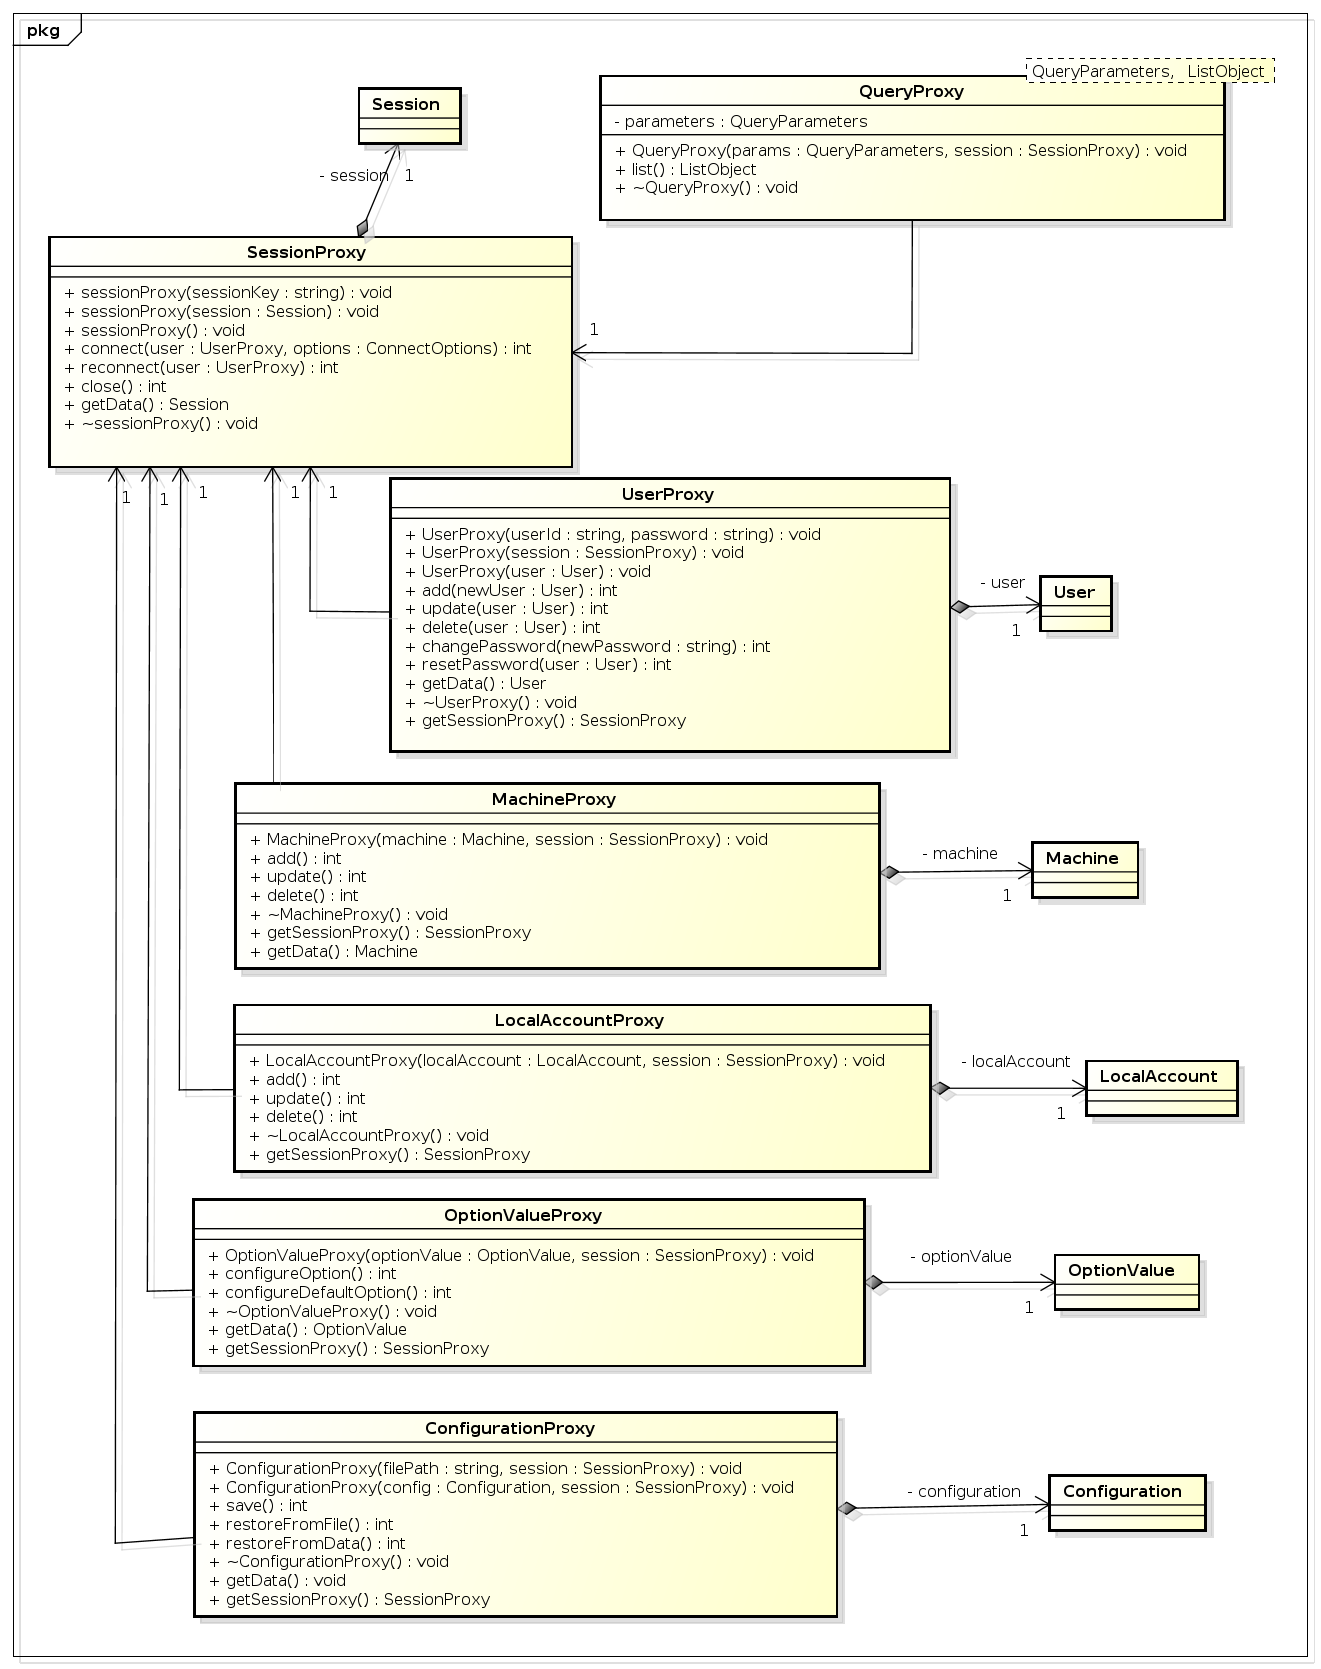
\includegraphics[scale=0.4]{images/png/UMS_Client_Class_Diagram.png}}}}{}
\end{center}
\caption{UMS Client Class Diagram}
\end{figure}

\section{UMS server modelization}

\subsection{Class diagrams}

\subsubsection{UMS Server Class Diagram}

This diagram presents the main objects used by UMS server component to process the UMS Client component requests. Each object that can be listed have a static method list with the corresponding options.
\begin{figure}[H]

\begin{center}
\imgexists{images/png/UMS_Server_Class_Diagram.png}{{\centering \imgevalsize{images/png/UMS_Server_Class_Diagram.png}{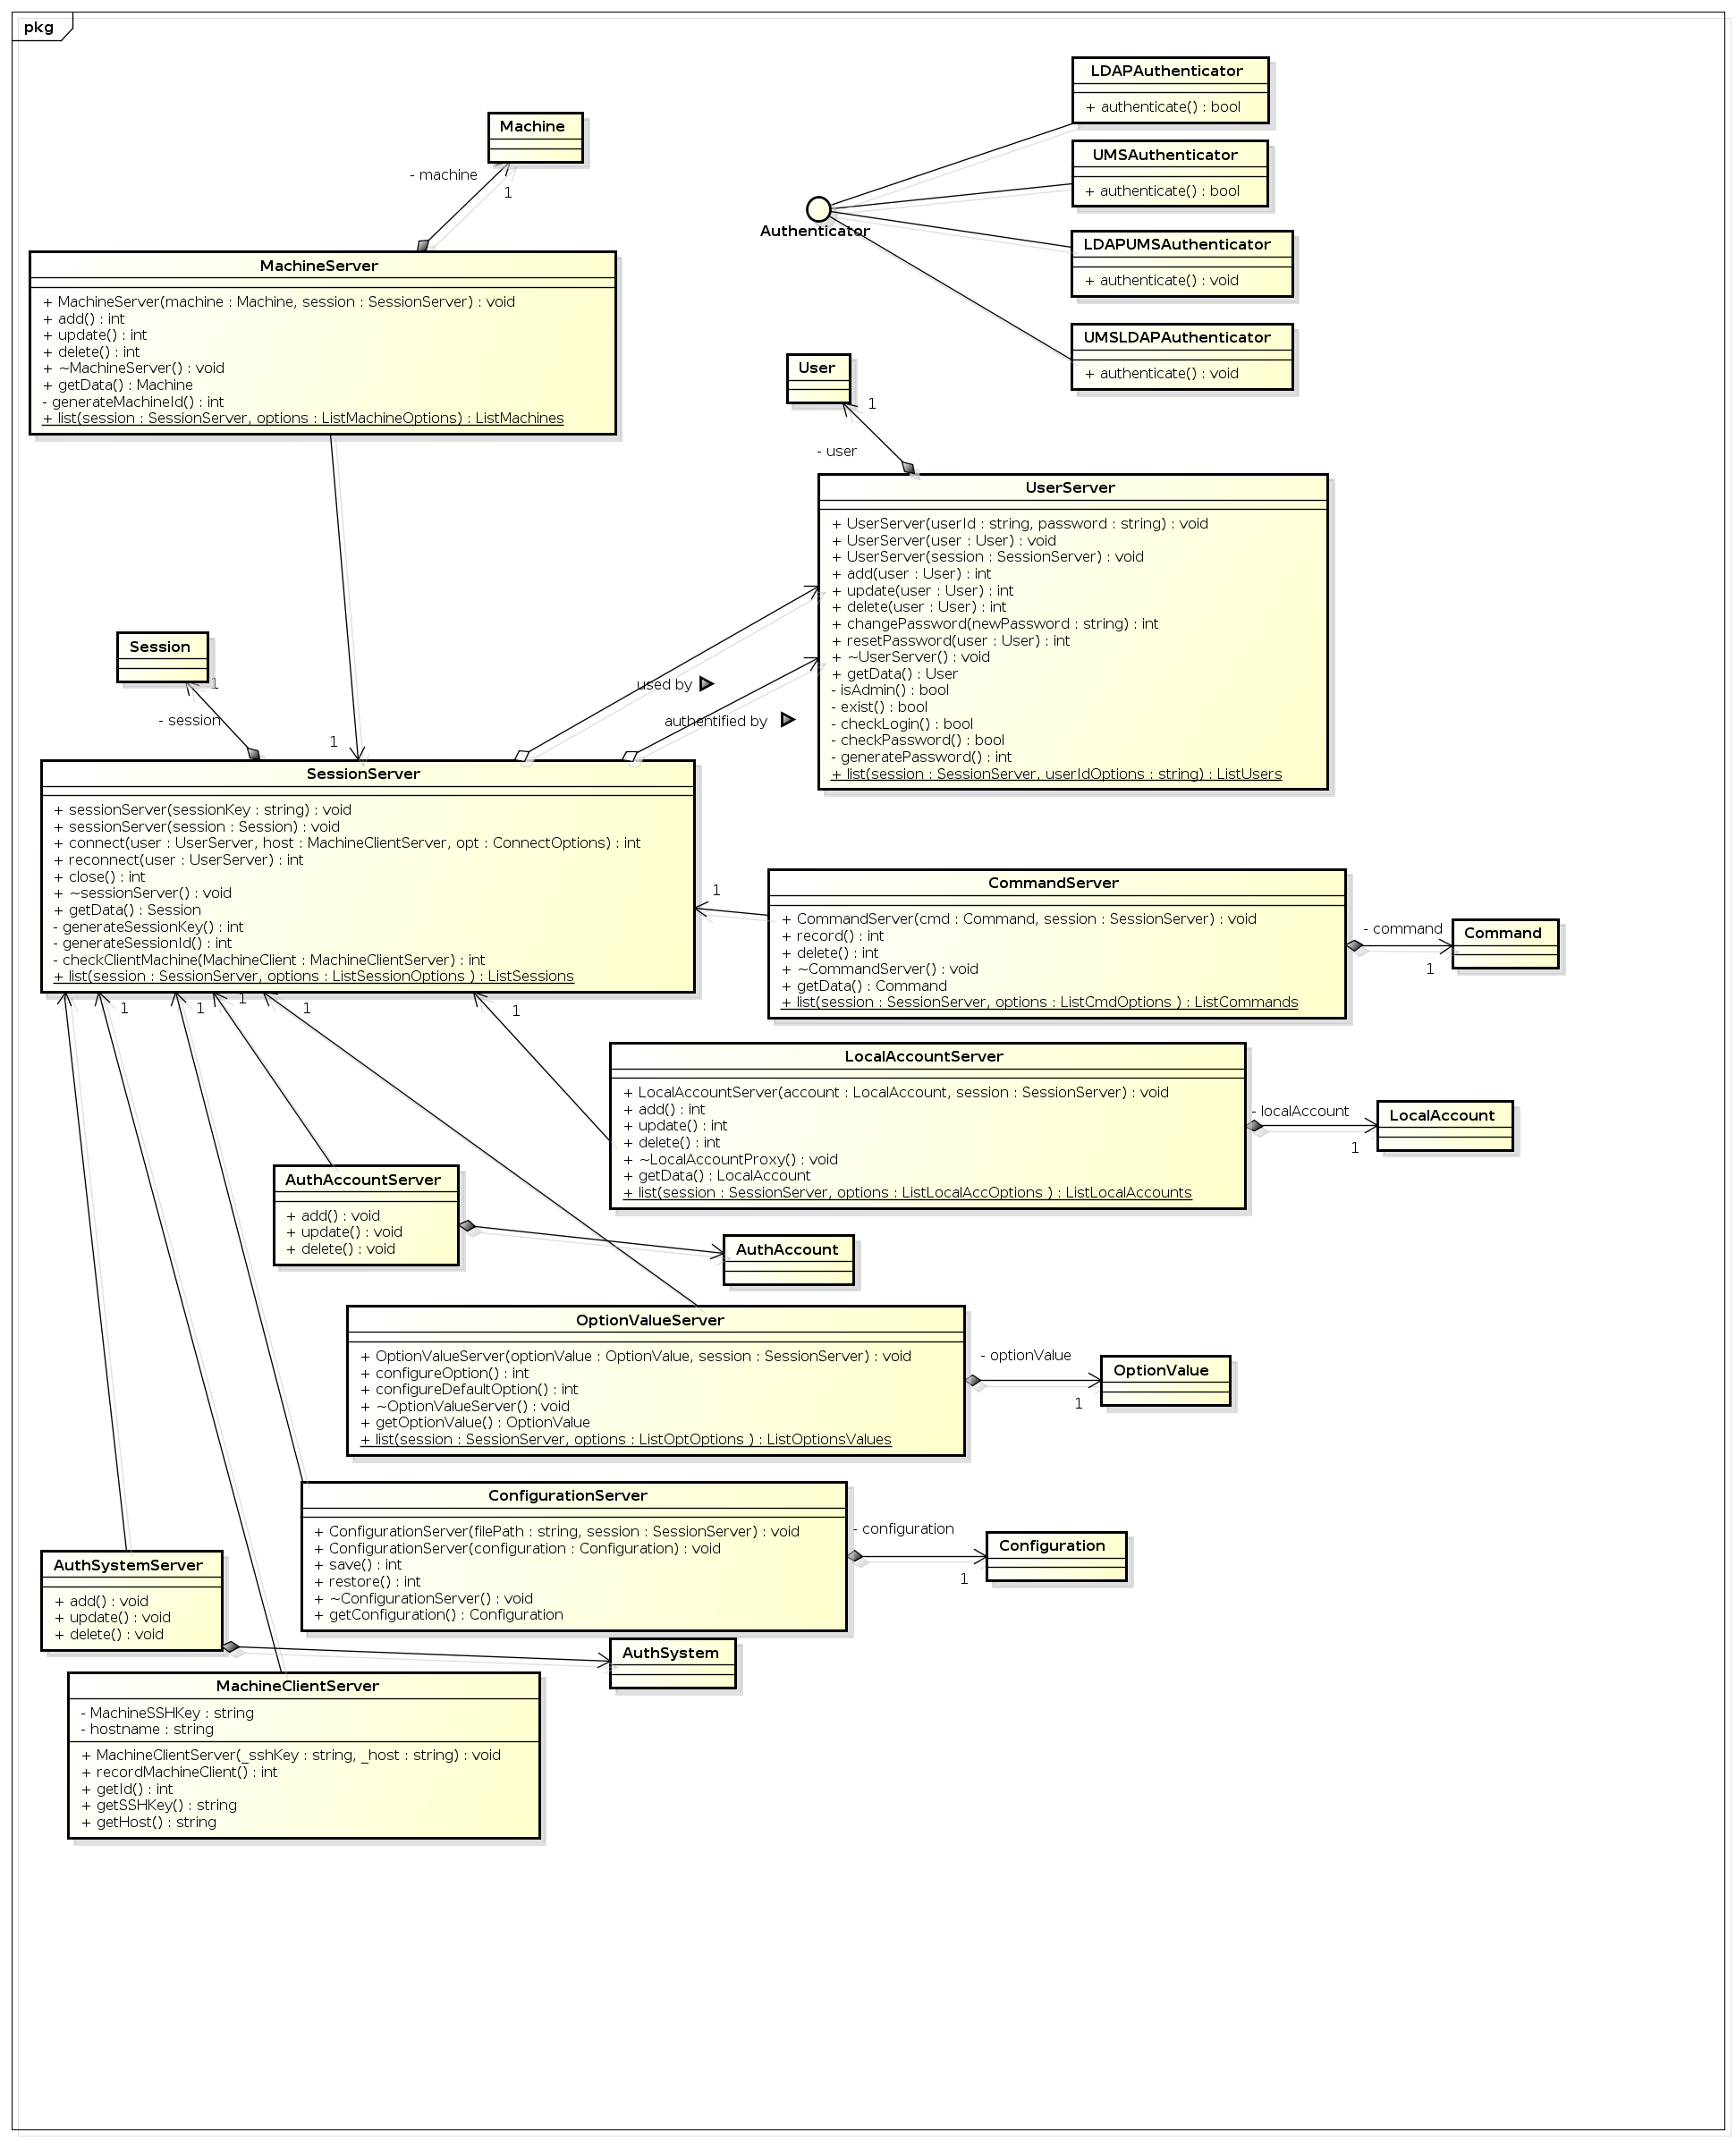
\includegraphics[scale=0.4]{images/png/UMS_Server_Class_Diagram.png}}}}{}
\end{center}
\caption{UMS Server Class Diagram}
\end{figure}

\section{UMS data modelization}

\subsection{Class diagrams}

\subsubsection{UMS Data Class Diagram}

This diagram illustrates the structure and the relationship between data manipulated by the components Client and Server. 
\begin{figure}[H]

\begin{center}
\imgexists{images/png/UMS_Data_Class_Diagram.png}{{\centering \imgevalsize{images/png/UMS_Data_Class_Diagram.png}{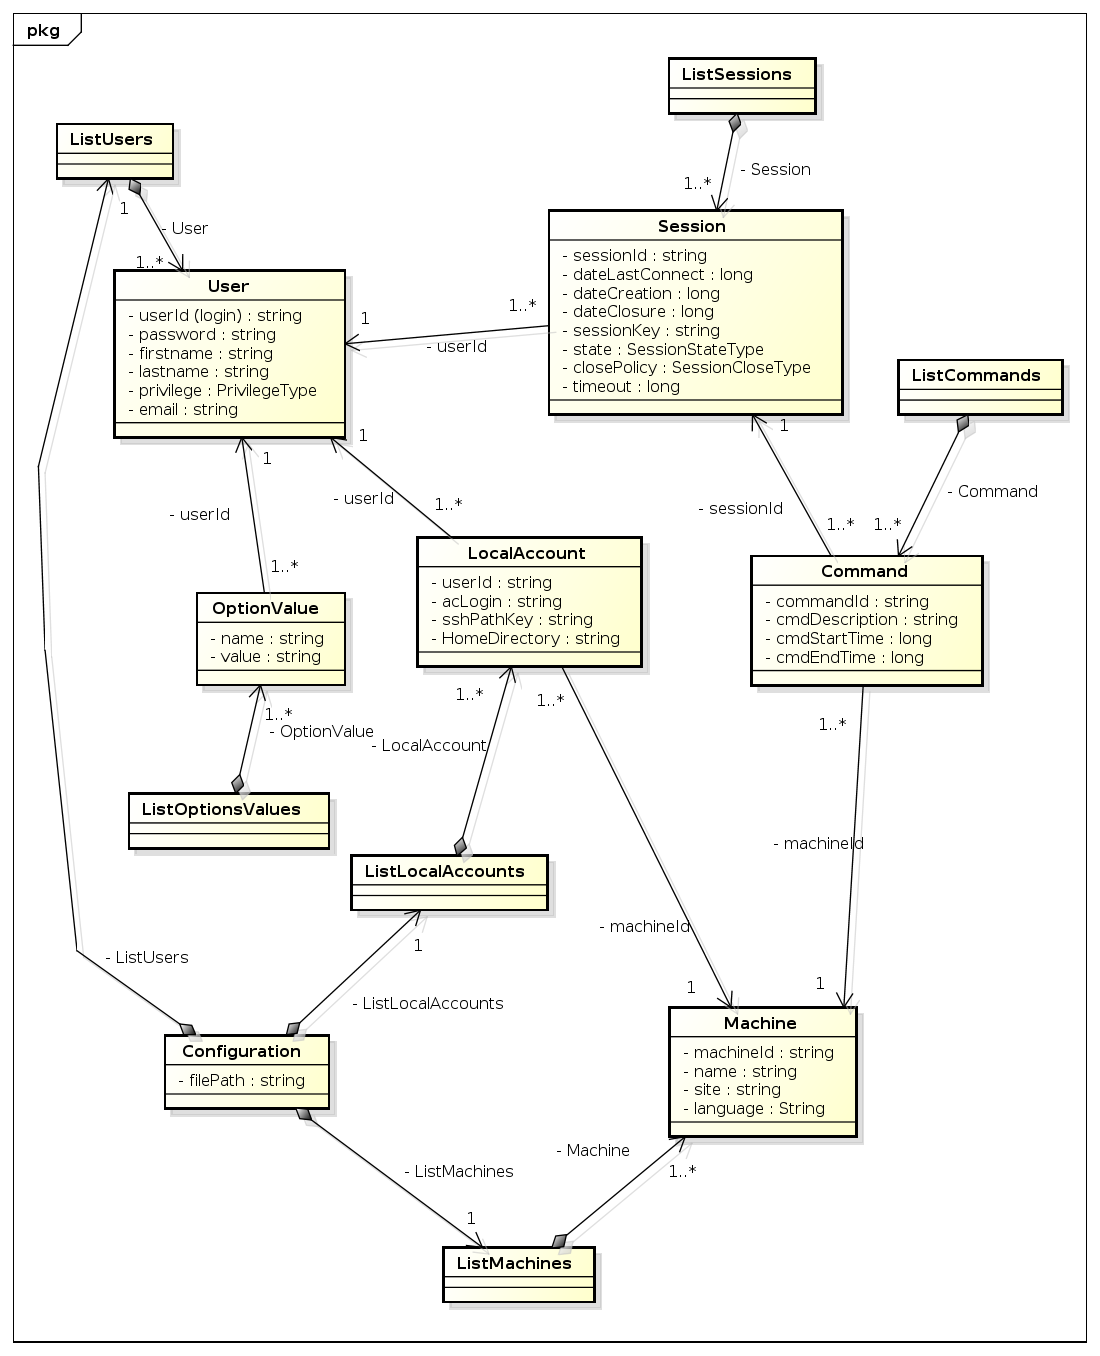
\includegraphics[scale=0.4]{images/png/UMS_Data_Class_Diagram.png}}}}{}
\end{center}
\caption{UMS Data Class Diagram}
\end{figure}

\section{Vishnu core functions modelization}

\subsection{Introduction}

 	The following elements describe the core classes (i.e. the classes that will be used by each module such as the exceptions and the databases). The modelization diagrams are given with some explanations about them.
 

\subsection{Tables relationships}

 	  In order to have a coherent System, we have designed a relational model for the database. We need only one database that can contain all the Vishnu tables. The model is represented in figure 4.4. The rectangles are the tables and the lines represent the links between the tables.
 

The links between the tables are based on the following rules:
 
\begin{itemize}

\item{}  
\begin{itemize}

\item{}The \emph{VISHNU} table has one or more \emph{MACHINE}  


\item{}A \emph{MACHINE} is in one and only one \emph{VISHNU} infrastructure
 

\end{itemize}


\item{}  
\begin{itemize}

\item{}A \emph{MACHINE} has one or more \emph{CPU}  


\item{} 		  A \emph{CPU} is in one and only one \emph{MACHINE}  

\end{itemize}


\item{}  
\begin{itemize}

\item{}A \emph{MACHINE} has one or more \emph{DESCRIPTION}  


\item{}A \emph{DESCRIPTION} is for one and only one \emph{MACHINE}  

\end{itemize}


\item{}   
\begin{itemize}

\item{}A \emph{MACHINE} has one or more \emph{THRESHOLD}  


\item{}A \emph{THRESHOLD} is for one and only one \emph{MACHINE}  

\end{itemize}


\item{}  
\begin{itemize}

\item{}A \emph{MACHINE} has one or more \emph{ACCOUNT}  


\item{}An \emph{ACCOUNT} is for one and only one \emph{MACHINE}  

\end{itemize}


\item{}  
\begin{itemize}

\item{}The \emph{VISHNU} table has one or more \emph{USER}  


\item{}An \emph{USER} is in one and only one \emph{VISHNU} infrastructure
 

\end{itemize}


\item{}  
\begin{itemize}

\item{}An \emph{USER} has one or more \emph{ACCOUNT}  


\item{}An \emph{ACCOUNT} is for one and only one \emph{USER}  

\end{itemize}


\item{}  
\begin{itemize}

\item{}An \emph{USER} has one or more \emph{FILE TRANSFER}  


\item{}A \emph{FILE TRANSFER} is for one and only one \emph{USER}  

\end{itemize}


\item{}  
\begin{itemize}

\item{}An \emph{USER} has one or more \emph{OPTION VALUE}  


\item{}An \emph{OPTION VALUE} is for one and only one \emph{USER}  

\end{itemize}


\item{}  
\begin{itemize}

\item{}An \emph{USER} sets one or more \emph{THRESHOLD}  


\item{}A \emph{THRESHOLD} is set by one and only one \emph{USER}  

\end{itemize}


\item{}  
\begin{itemize}

\item{}An \emph{OPTION} has one or more \emph{OPTION VALUE}  


\item{}An \emph{OPTION VALUE} is for one and only one \emph{OPTION}  

\end{itemize}


\item{}  
\begin{itemize}

\item{}An \emph{USER} has one or more \emph{SESSION}  


\item{}A \emph{SESSION} is for one and only one \emph{USER}  

\end{itemize}


\item{}  
\begin{itemize}

\item{}A \emph{SESSION} has one or more \emph{COMMAND}  


\item{}A \emph{COMMAND} is for one and only one \emph{SESSION}  

\end{itemize}


\item{}  
\begin{itemize}

\item{}A \emph{CLIENT MACHINE} has one or more \emph{SESSION}  


\item{}A  \emph{SESSION}  is  for  one  and  only  one  \emph{CLIENT
		    MACHINE}  

\end{itemize}


\item{}  
\begin{itemize}

\item{}A \emph{MACHINE} has one or more \emph{STATE}  


\item{}A \emph{STATE} is for one and only one \emph{MACHINE}  

\end{itemize}


\item{}  
\begin{itemize}

\item{}A \emph{COMMAND} can have one or more \emph{JOB}  


\item{}A \emph{JOB} is for one and only one \emph{COMMAND}  

\end{itemize}


\item{}  
\begin{itemize}

\item{}A \emph{COMMAND} can have one or more \emph{FILE}  


\item{}A \emph{FILE} is for one and only one \emph{COMMAND}  

\end{itemize}

\end{itemize}

\subsection{Relational model}
\begin{figure}[H]

\begin{center}
\imgexists{images/png/relationnalmodel.png}{{\centering \imgevalsize{images/png/relationnalmodel.png}{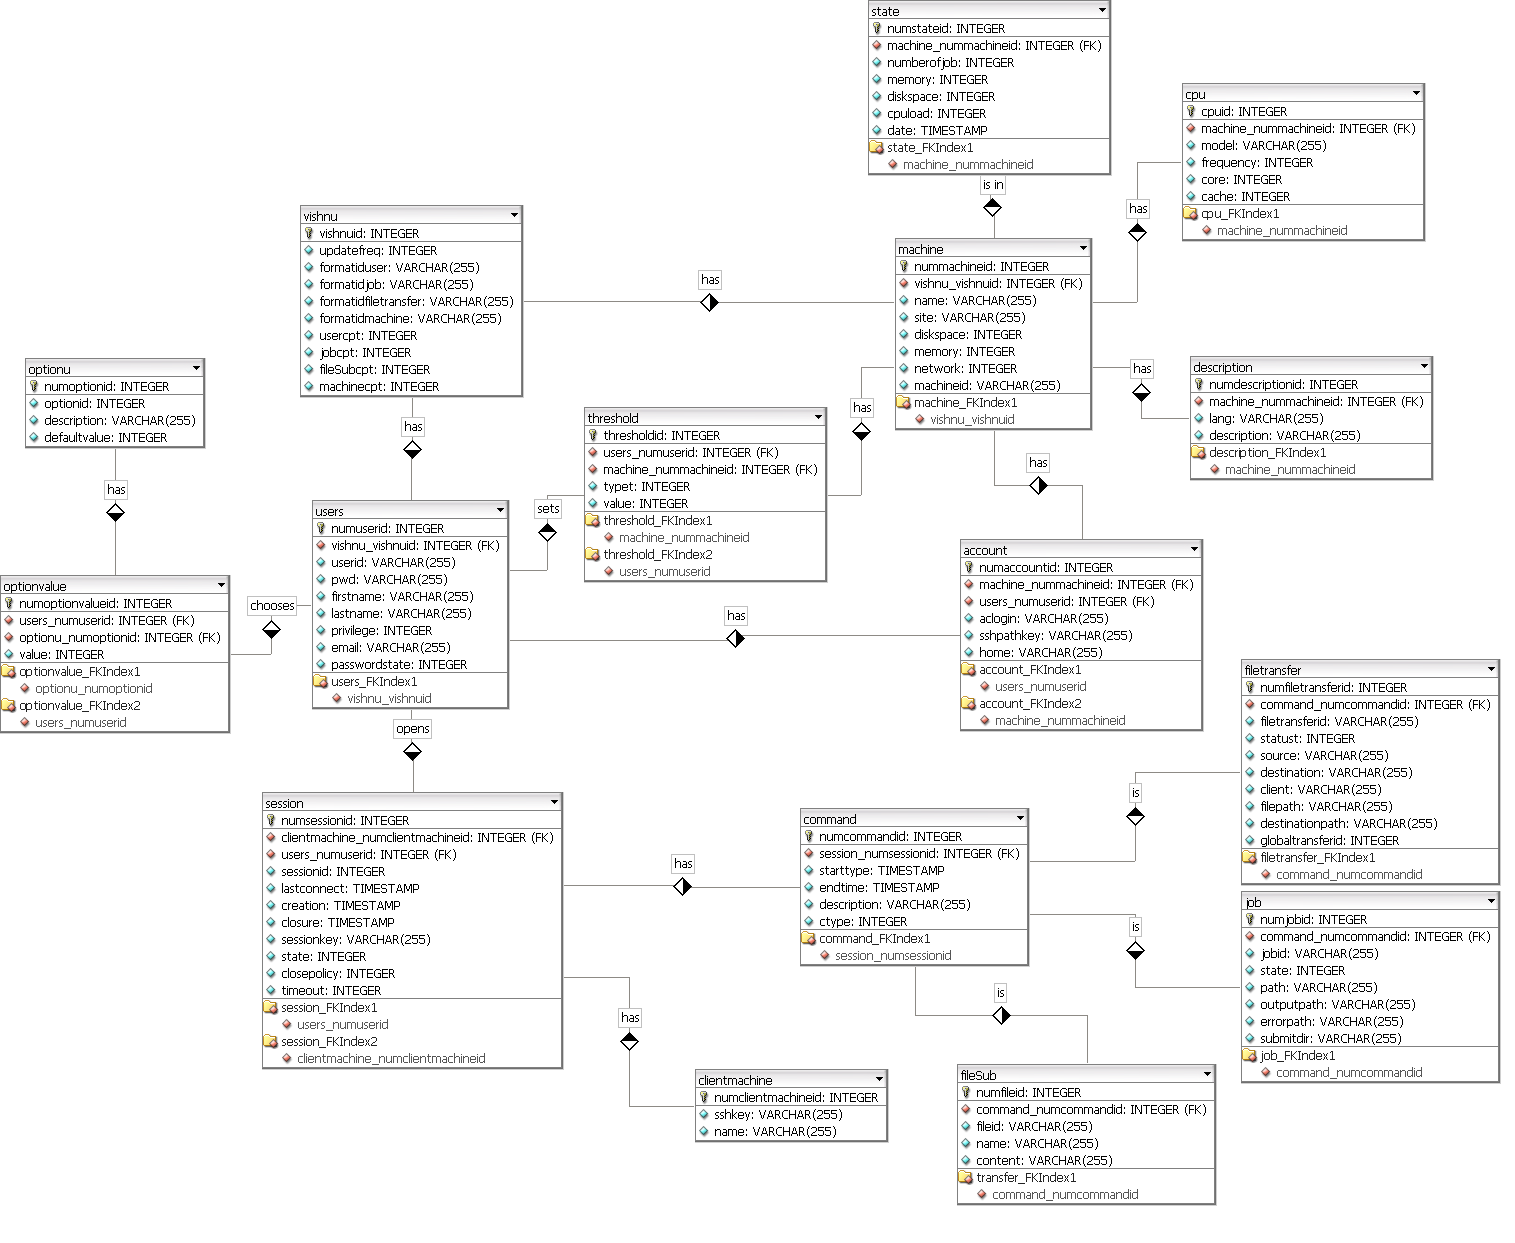
\includegraphics[scale=0.4]{images/png/relationnalmodel.png}}}}{}
\end{center}
\caption{Relational model}
\end{figure}

\subsection{ 	  The modelization
 }

\subsubsection{The database classes}

 	    The database class diagram is very simple. There is a database interface that defines a set of public operations that can be done over a database:
 \begin{itemize}

\item{} 		  commit
 


\item{} 		  rollback
 


\item{} 		  execute a query
 


\item{} 		  connect
 


\item{} 		  disconnect ...
 

\end{itemize}
 	    And there are two examples of classes that implement the database. There is also a factory that can create the databases.
	    See the diagram 4.5.
 

\subsubsection{The exception classes}

 	    The exception class diagram defines a generic exception class, \emph{VishnuException} that represents a generic exception that can be raised by a Vishnu function. This class has two subclasses, the \emph{SystemException} that represents an exception due to a system problem and the \emph{UserException} that represents an exception due to the user of the function (bad parameters typically). Both the server and clients have this way of building the exceptions. The \emph{SystemException} has more specific subclasses depending on the modules that raises them. A key function is the append one, that allows to add a message to an existing vishnu exception. Thus, crossing the various level of the call can append information messages to specify the context of the exception.
	    See the diagram 4.6.
 

\subsection{Class diagrams}

\subsubsection{DB class diagram}
\begin{figure}[H]

\begin{center}
\imgexists{images/png/DB_class_diagram.png}{{\centering \imgevalsize{images/png/DB_class_diagram.png}{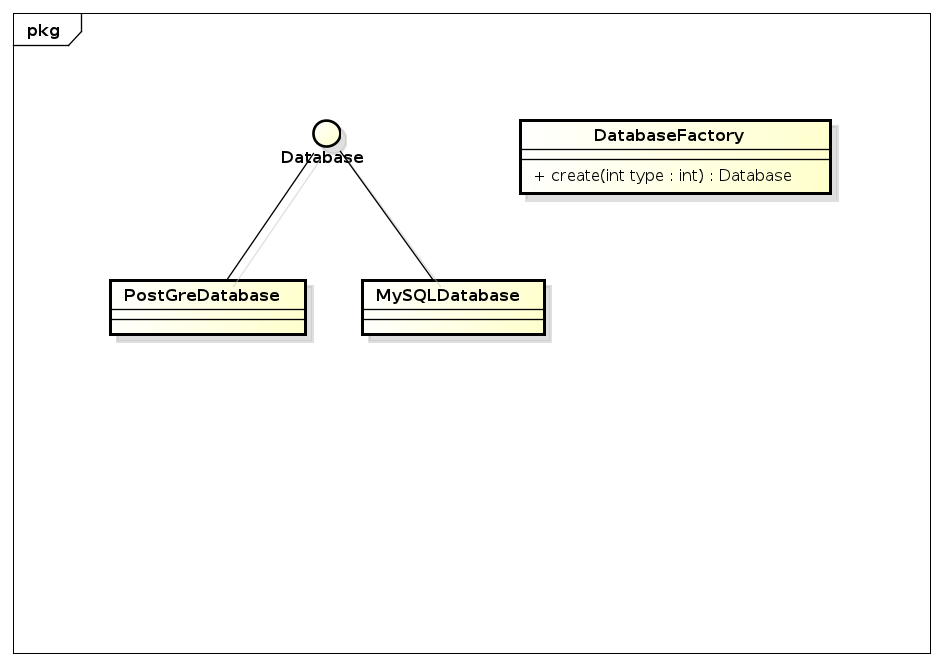
\includegraphics[scale=0.4]{images/png/DB_class_diagram.png}}}}{}
\end{center}
\caption{DB class diagram}
\end{figure}

\subsubsection{exception}
\begin{figure}[H]

\begin{center}
\imgexists{images/png/exception.png}{{\centering \imgevalsize{images/png/exception.png}{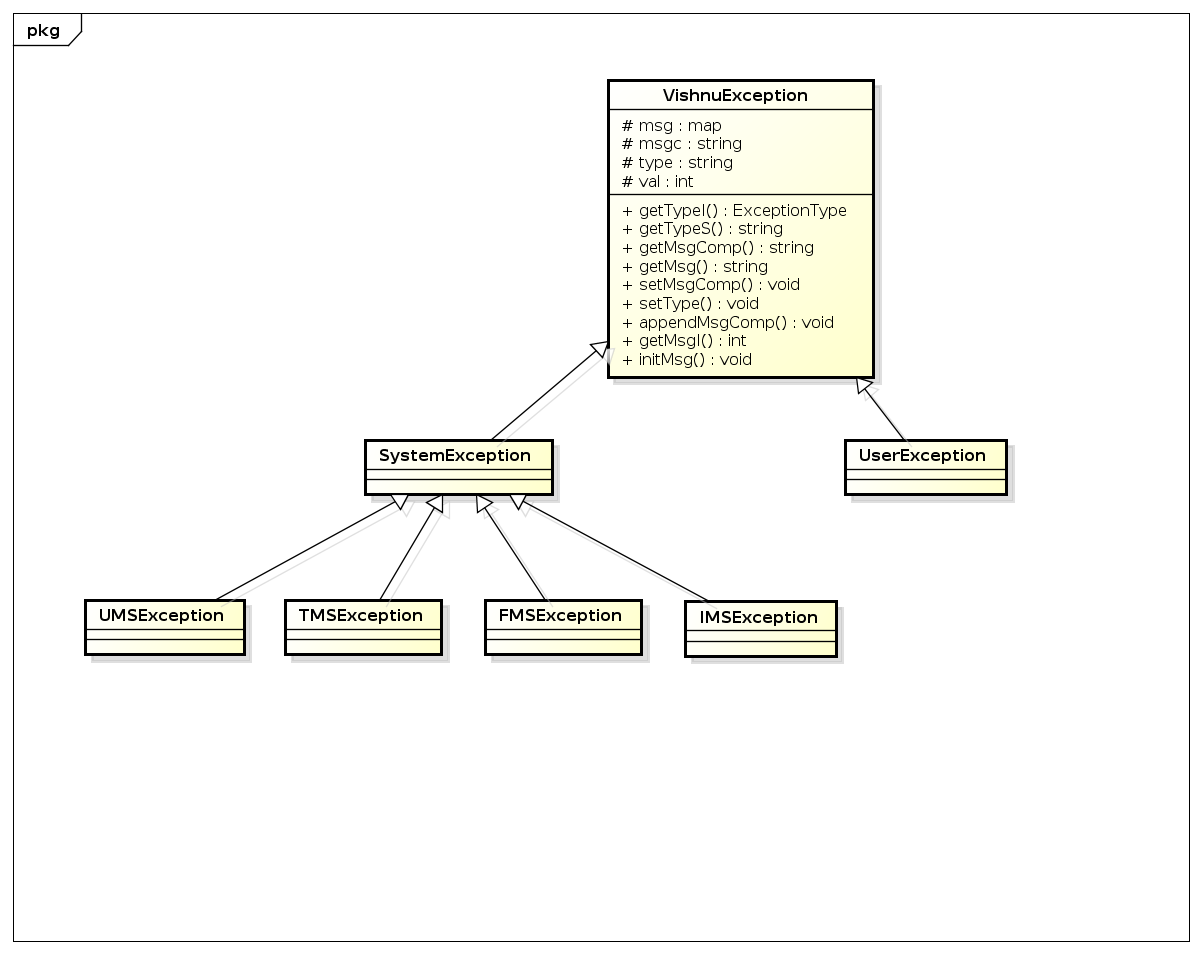
\includegraphics[scale=0.4]{images/png/exception.png}}}}{}
\end{center}
\caption{exception}
\end{figure}

\end{document}
